\documentclass[10pt,twocolumn,a4paper]{article}

% ---------------------------------------------------------------
%  Coca Is Not Cocaine — two-column academic paper (English)
%  Compile with: latexmk -pdf coca.tex
% ---------------------------------------------------------------

\usepackage[T1]{fontenc}
\usepackage[utf8]{inputenc}
\usepackage[english]{babel}
\usepackage{lmodern}
\usepackage{microtype}
\usepackage[a4paper,margin=1.8cm,columnsep=0.7cm]{geometry}
\usepackage{graphicx}
\usepackage{booktabs}
\usepackage{array}
\usepackage{amsmath,amssymb}
\usepackage[round,authoryear]{natbib}
\usepackage{caption}
\usepackage{subcaption}
\usepackage{enumitem}
\usepackage{xcolor}
\usepackage{textcomp}
\usepackage{balance}
\usepackage[hidelinks,colorlinks=true,linkcolor=violet,citecolor=violet,urlcolor=violet]{hyperref}

\graphicspath{{figs/}}
\captionsetup{font=small,labelfont=bf}
\setlength{\parindent}{1em}

% Auxiliary commands
\newcommand{\code}[1]{\texttt{\small #1}}
\newcommand{\concept}[1]{\emph{#1}}
\newcommand{\Fone}{\textbf{F1}}
\newcommand{\Ftwo}{\textbf{F2}}
\newcommand{\Fthree}{\textbf{F3}}

\begin{document}

% ---------- Full-width title + abstract ----------
\twocolumn[{%
\vspace{-0.5em}
\begin{center}
  {\LARGE\bfseries Coca Is Not Cocaine}\\[0.45em]
  {\large Three Lexical-Cultural Collision Modes in Open-Weight LLMs, Probed in Catalan}\\[1.1em]
  {\large Xavier Vinaixa Roselló}\\[0.35em]
  {\small Sorensen AI, Barcelona, Catalonia}\\[0.15em]
  {\small ORCID 0009-0005-2769-9215 \quad\textbar\quad \texttt{xavi@sorensen.ai}}\\[0.4em]
  {\small 2026 \quad\textbar\quad \textit{Preprint --- not peer-reviewed}}\\[0.25em]
  {\small DOI: \href{https://doi.org/10.13140/RG.2.2.10368.39682}{10.13140/RG.2.2.10368.39682}}
\end{center}
\vspace{0.8em}
\begin{center}
\begin{minipage}{0.86\textwidth}
\small
\noindent\textbf{Abstract.}
Culturally-marked Catalan concepts collide with the Anglo-Saxon imaginary in
at least three structurally distinct ways, and naive cultural-bias probes
conflate them into a single number. A \concept{gegant} is not a fairy-tale
\emph{giant} (it is a festive effigy), a \concept{coca} is not cocaine (it is
a flatbread), and a \concept{pinya} at the base of a \concept{castell} is
neither a pinecone nor a pineapple. We extend the CAMeL framework
\citep{naous2024} to a panel of \textbf{eleven open-weight base LLMs} through
contextualized hidden-state geometry --- mean-pooled, L2-normalized vectors
at a best layer chosen by KNN purity over anchors --- and stratify the bias
ratio $\text{pull}_{\text{anglo}} / (\text{pull}_{\text{anglo}} +
\text{pull}_{\text{catalan}})$ along an \code{ambiguity\_type} axis. This
separates (i) cross-lingual cognate drag (\concept{gegant}, \concept{castell},
\concept{coca}), (ii) purely domain-specific representation gaps
(\concept{correfoc}, \concept{casteller}, \concept{romesco}), and (iii)
intra-Catalan polysemy (\concept{pinya}, \concept{tió}, \concept{folre},
\concept{manilles}). The panel pairs four general-purpose families (Gemma,
Qwen, Mistral, DeepSeek) with a Catalan-aware control tier (Salamandra/ALIA
from the Barcelona Supercomputing Center). The central result is that all five
families exhibit the \textbf{same collision pattern} in the absence of
context, which locates the cause of the collision in the
\emph{contextualized-embedding pipeline} rather than in the training-data
mixture. A pre-registered title test confirms that the literal reading
---\concept{coca} adjacent to \emph{cocaine}, \emph{Coca-Cola}, \emph{coke}---
is a property of latent space in ten of eleven models. The practical
intervention is complementary to any pretraining strategy: supply Catalan
context in the inference-time prompt.

\medskip
\noindent\textbf{Keywords:} cultural bias, LLM, Catalan, contextualized
embeddings, low-resource languages, Salamandra, ALIA.
\end{minipage}
\end{center}
\vspace{1.0em}
}]

% ---------------------------------------------------------------
\section{Introduction}
% ---------------------------------------------------------------

Large language models (LLMs) are trained on corpora massively dominated by
English. A known consequence is cultural misalignment: models systematically
reproduce the Western --- and especially Anglo-Saxon --- imaginary when asked
to reason about non-anglophone societies \citep{tao2024,wang2023,adalovelace2025}.
Most existing cultural-bias probes measure this with a single aggregate number
\citep{naous2024,li2023}, which hides the fact that a culturally-marked concept
can fail in qualitatively different ways.

This work takes Catalan as a limiting case and asks a concrete, measurable
question: \emph{when a base LLM reads a culturally-marked Catalan word, where
does it place it in latent space?} A \concept{coca} is a sweet or savoury
flatbread typical of Catalan cuisine; in English, \emph{coca} points to the
plant, the drug, or the soft-drink brand. A \concept{gegant} is a festive
papier-mâché figure that parades through town squares; its English cognate
\emph{giant} lives in a fairy-tale universe. And a \concept{pinya} can be a
pinecone, a pineapple, or the human base of a \concept{castell} (human tower),
depending on context.

We argue that these three examples illustrate three \emph{structurally
distinct failure modes}, which we call \Fone{}, \Ftwo{} and \Fthree{}
(Section~\ref{sec:taxonomy}), and that they deserve different diagnostics ---
and interventions. The central contribution is methodological: we show that
stratifying the bias metric by ambiguity type reveals stories that the
aggregate metric hides.

\paragraph{Contributions.}
\begin{enumerate}[leftmargin=1.4em,itemsep=2pt,topsep=2pt]
  \item A \textbf{three-mode taxonomy} (\Fone{}/\Ftwo{}/\Fthree{}) of
        lexical-cultural collisions, with a hand-curated 56-concept Catalan
        lexicon stratified by ambiguity type.
  \item A \textbf{geometric adaptation of CAMeL} \citep{naous2024} from
        fill-in-the-blank to contextualized-embedding geometry, with bootstrap
        confidence intervals per (concept, frame).
  \item An \textbf{eleven-model base panel} pairing four general-purpose
        families with a \textbf{causal Catalan-aware control} (Salamandra/ALIA
        from the BSC), which lets us distinguish the ``the problem is the
        data'' hypothesis from the ``the problem is the pipeline'' hypothesis.
  \item A \textbf{pre-registered title test} that literally validates the
        \concept{coca}~$\leftrightarrow$~\emph{cocaine} collision in latent
        space.
\end{enumerate}

\begin{figure*}[t]
  \centering
  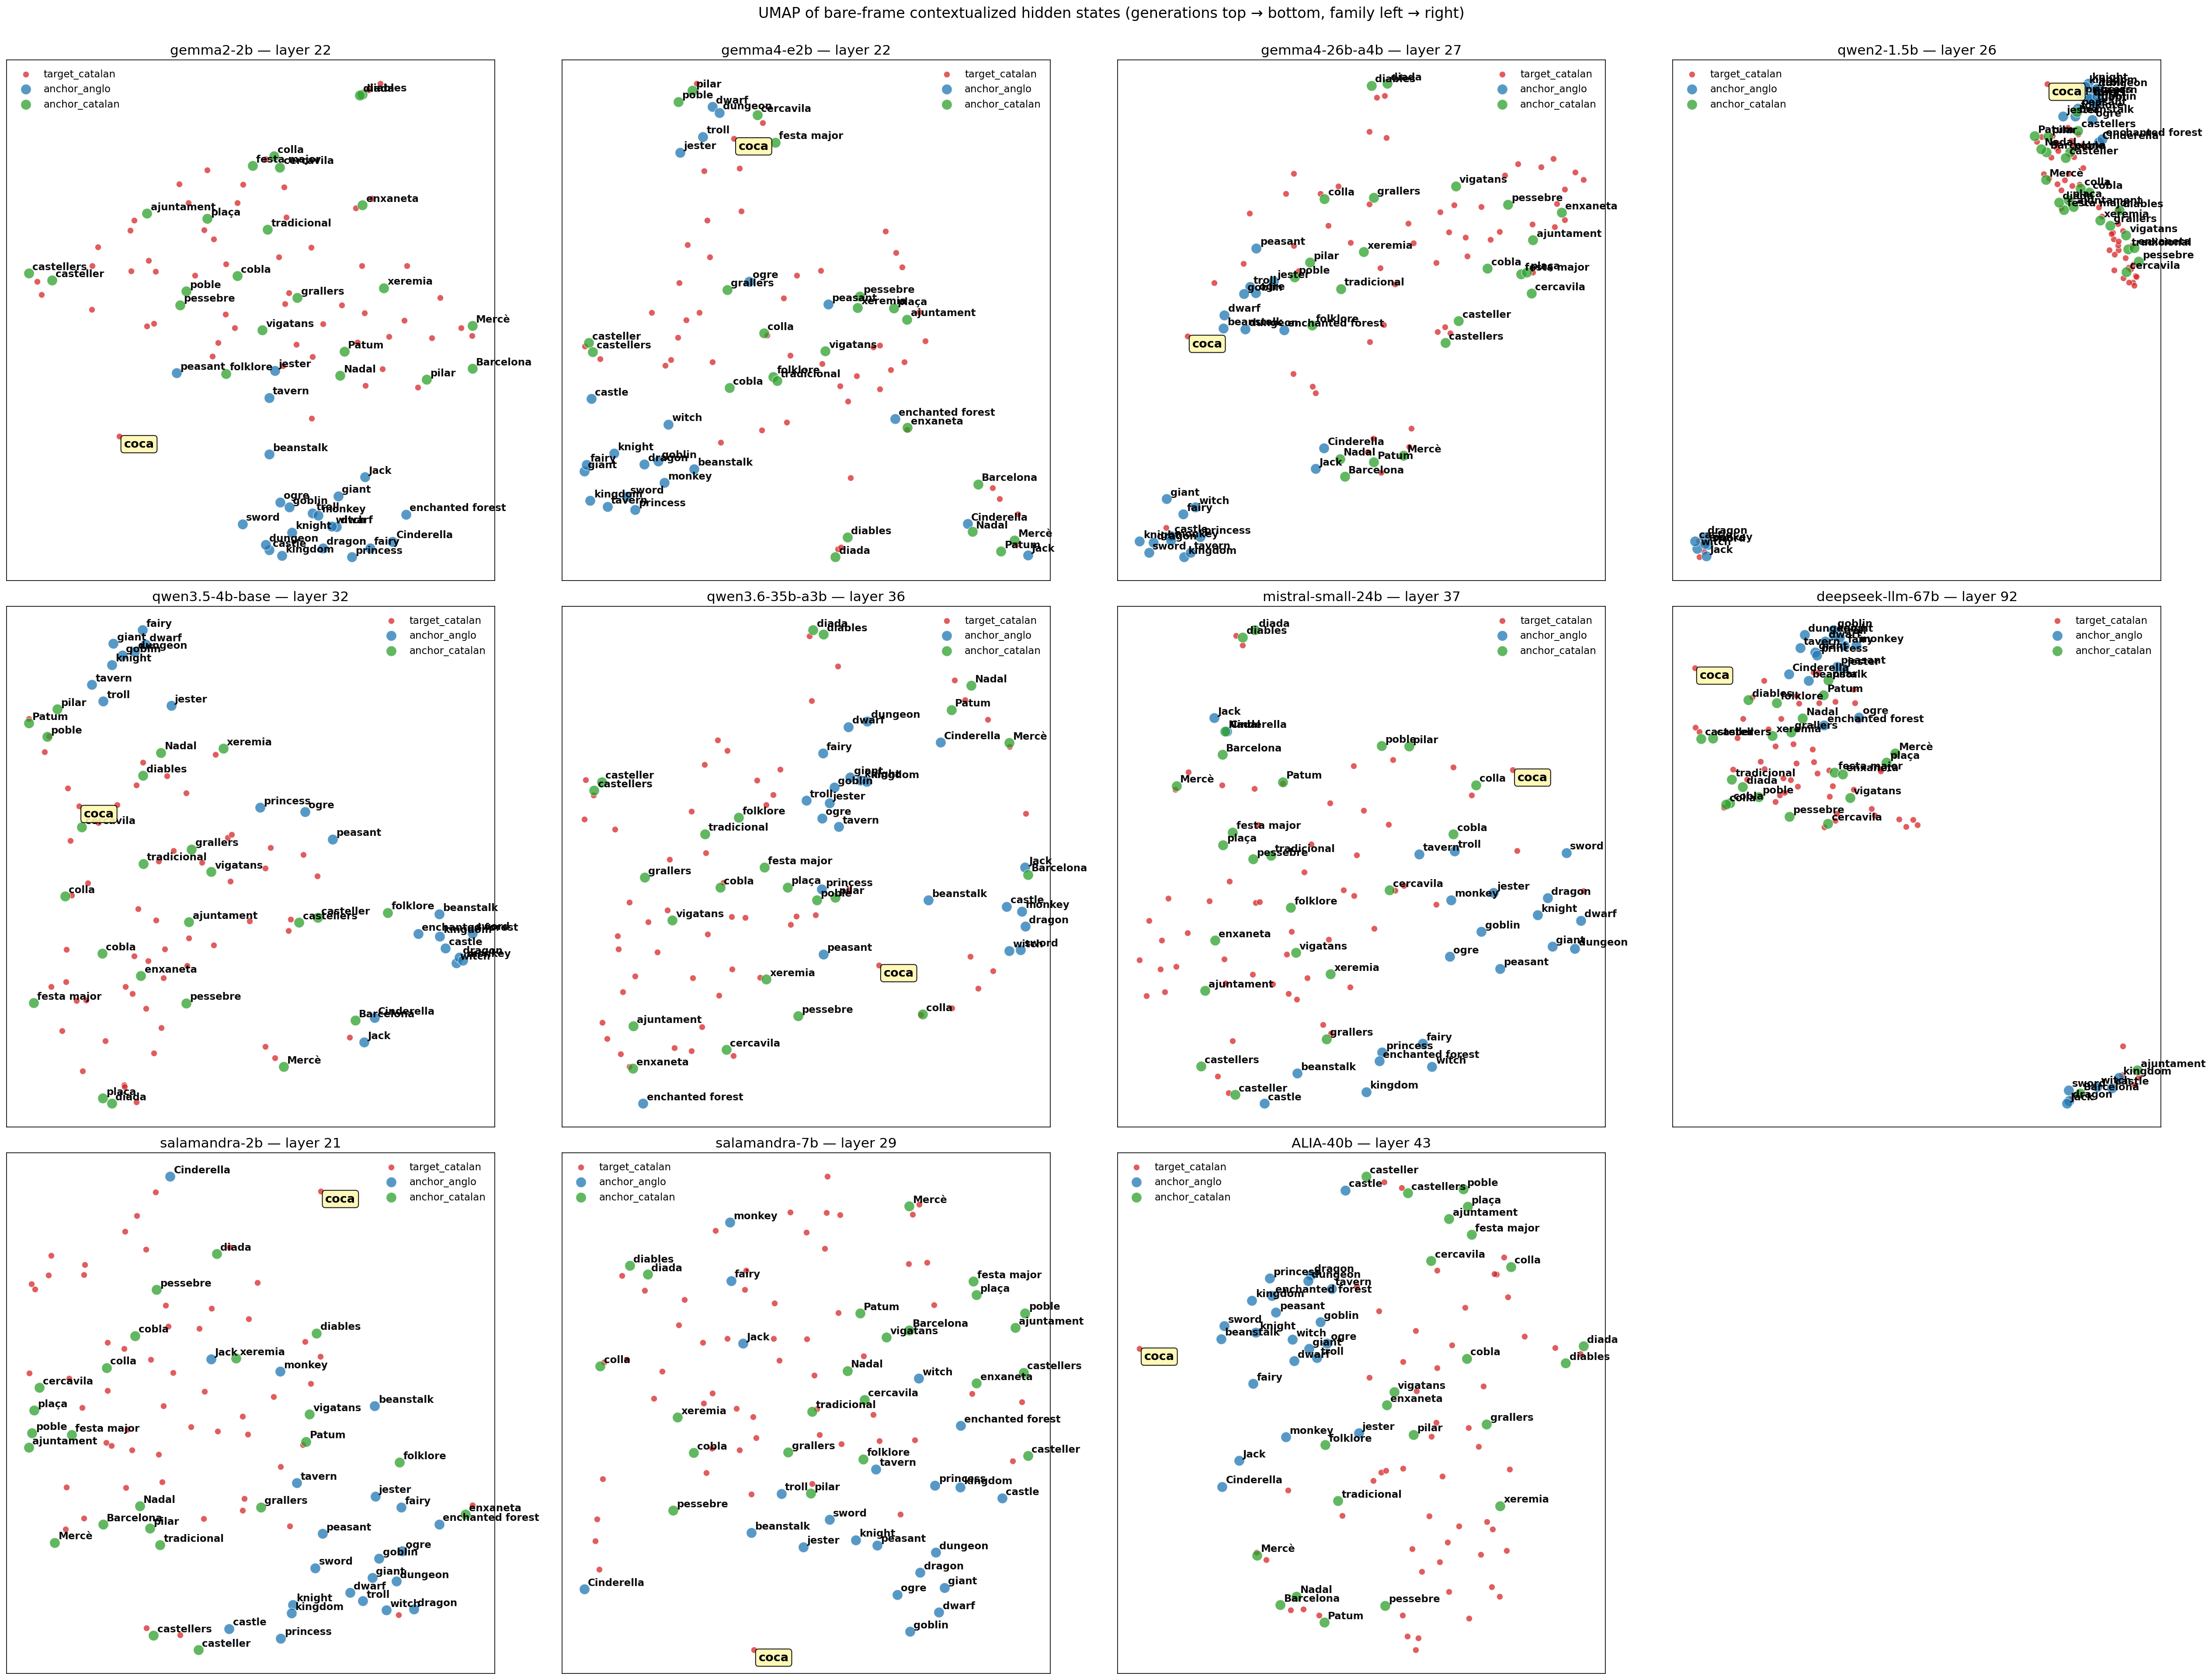
\includegraphics[width=0.92\textwidth]{headline_umap.png}
  \caption{UMAP of the contextualized hidden states in the \code{bare} frame
  at each model's best layer, in a grid ordered by family (Gemma
  $\rightarrow$ Qwen $\rightarrow$ Mistral $\rightarrow$ DeepSeek
  $\rightarrow$ Salamandra $\rightarrow$ ALIA) and then by size. \concept{coca}
  is highlighted with a yellow callout in every panel: following it across
  models shows the title concept's journey through eleven different latent
  spaces.}
  \label{fig:headline}
\end{figure*}

% ---------------------------------------------------------------
\section{Related work}\label{sec:related}
% ---------------------------------------------------------------

\paragraph{Direct methodological inspiration.}
The reference framework is \textbf{CAMeL} \citep{naous2024}, which measures
cultural bias with fill-in-the-blank probes in Arabic. This project takes it
(i) from fill-in-the-blank to contextualized-embedding geometry, (ii) from
Arabic to Catalan, and (iii) adds the \Fone{}/\Ftwo{}/\Fthree{} taxonomy that
separates the failure modes CAMeL aggregates into a single metric.

\paragraph{The cultural-bias trunk.}
\citet{tao2024} show systematic cultural misalignment in LLM outputs about
non-Western societies --- the macro ``why it matters'' behind our
micro-geometric work. \citet{li2023} (GeoMLAMA) confirm that the problem cuts
across probe modalities. \citet{rystrom2025} argue that training on more
languages does not imply capturing more cultures (\emph{multilingual $\neq$
multicultural}): this is exactly the ``pipeline, not data-mix'' reading that
the Salamandra/ALIA family confirms empirically here. \citet{wang2023}
document Anglo-American cultural dominance in the training mix, the direct
motivation for using Catalan as a limiting case.

\paragraph{Classic embedding-geometry tradition.}
\citet{bolukbasi2016} is the founding work on bias probes via cosine
proximity to anchor sets. Our
$\text{bias\_ratio} = \text{pull}_{\text{anglo}}/(\text{pull}_{\text{anglo}}
+ \text{pull}_{\text{catalan}})$ is its contextualized extension, applied to a
cultural collision rather than a gender collision.

\paragraph{Methodological constraint.}
\citet{dettmers2022} show that quantization reorganizes representation
geometry. This grounds the ``bf16 only, no fp8 / int8 / NVFP4'' rule applied
across the whole panel (Section~\ref{sec:extraction}).

% ---------------------------------------------------------------
\section{The F1/F2/F3 taxonomy}\label{sec:taxonomy}
% ---------------------------------------------------------------

A culturally-marked target word $c$ in a low-resource language can fail in
three structurally distinct ways when a probe asks where $c$ sits in a
multilingual base LLM's latent space. The 56-concept lexicon
(\code{data/concepts\_ca.csv}) is stratified by an \code{ambiguity\_type}
column that tags each target with exactly one of the codes in
Table~\ref{tab:taxonomy}.

\begin{table*}[t]
  \centering
  \small
  \renewcommand{\arraystretch}{1.35}
  \begin{tabular}{@{}clcp{9.6cm}@{}}
    \toprule
    \textbf{Code} & \textbf{Type} & \textbf{n} & \textbf{Failure mode / examples} \\
    \midrule
    \Fone{} & \code{cross\_lingual\_bias} & 10 &
      Direct English cognate, different universe.
      \concept{gegant}$\leftrightarrow$giant, \concept{castell}$\leftrightarrow$castle,
      \concept{drac}$\leftrightarrow$dragon, \concept{coca}$\leftrightarrow$coca,
      \concept{Pasqua}$\leftrightarrow$Easter. \\
    \Ftwo{} & \code{domain\_specific} & 29 &
      No English cognate --- pure domain depth.
      \concept{correfoc}, \concept{casteller}, \concept{cercavila},
      \concept{panellet}, \concept{grallers}, \concept{pa amb tomàquet},
      \concept{samfaina}, \concept{calçotada}, \concept{romesco}. \\
    \Fthree{} & \code{internal\_polysemy} & 17 &
      Mundane Catalan sense dominates the festive one.
      \concept{pinya} (pinecone $\|$ castell base),
      \concept{tió} (log $\|$ Christmas log),
      \concept{folre} (lining $\|$ castell padding),
      \concept{manilles} (handcuffs $\|$ castell grip). \\
    \bottomrule
  \end{tabular}
  \caption{The three-mode taxonomy of lexical-cultural collisions.}
  \label{tab:taxonomy}
\end{table*}

\paragraph{Why each stratum needs a different intervention.}
\begin{itemize}[leftmargin=1.3em,itemsep=3pt,topsep=2pt]
  \item \Fone{} confounds \emph{anglification} with \emph{cognate semantics}:
        when \concept{gegant} lands near \emph{giant}, that is partly because
        they share an English referent and partly because English-dominant
        pretraining drags the Catalan word toward its cognate. A pull is
        observed but its cause is ambiguous by construction.
  \item \Ftwo{} is the cleanest evidence stratum. \concept{Correfoc} has no
        English cognate; if it lands inside the Anglo fairy-tale cluster the
        pull is structural --- there is no lexical shortcut to fall onto.
  \item \Fthree{} can produce a high pull \emph{without} anglification: if
        \concept{pinya} lands near \emph{pinecone}, the model is just
        reflecting that the mundane Catalan sense (the fruit) is more frequent
        in the training mix than the festive one (the castell base). The fix
        is not ``teach the model that \concept{pinya} $\neq$ \emph{giant}''; it
        is ``teach the model that \concept{pinya} has a second sense that is
        not a pinecone''.
\end{itemize}

\paragraph{F1 audit.}
\Fone{} is deliberately kept \emph{tight} (10 concepts) and conservative. A
concept enters \Fone{} only if it has a direct English cognate \textbf{and}
that cognate lives in a clearly different cultural universe. The audit removed
three concepts (\concept{mare}, \concept{port}, \concept{vall}) whose cognates
were culturally co-extensive with their Catalan senses, and moved
\concept{terra} from \Fone{} to \Fthree{} because its interesting case
(\emph{la terra} as political territory vs.\ \emph{terra} as soil) is
intra-Catalan polysemy rather than cross-lingual collision.

% ---------------------------------------------------------------
\section{Methodology}\label{sec:method}
% ---------------------------------------------------------------

\subsection{Probe-frame design}

For each target concept $c$ the pipeline emits four probes
(Table~\ref{tab:frames}). We deliberately leave the Catalan lemma verbatim in
\code{anglo\_en} even when $c$ has a direct English cognate: substituting
\concept{gegant}$\rightarrow$\emph{giant} would measure \emph{giant}'s
geometry, not the cross-lingual pull on \concept{gegant}.

\begin{table}[t]
  \centering
  \small
  \begin{tabular}{@{}lp{5.5cm}@{}}
    \toprule
    \textbf{\code{frame\_id}} & \textbf{Sentence} \\
    \midrule
    \code{bare}          & \concept{c} alone, no context. \\
    \code{anglo\_en}     & \emph{Once upon a time, there was a c who lived in the enchanted forest.} \\
    \code{catalan\_frame}& \emph{A la festa major del poble, els c van sortir a la plaça acompanyats dels grallers.} \\
    \code{neutral\_ca}   & \emph{El c és un element important.} \\
    \bottomrule
  \end{tabular}
  \caption{The four probe frames.}
  \label{tab:frames}
\end{table}

\subsection{Anchor sets}

Three hand-curated clusters are used: Anglo fairy-tale / medieval vocabulary
(22 entries, the dominant cluster), Catalan folkloric vocabulary (23 entries,
the target cluster), and a drug / brand / beverage cluster (13 entries, used
\emph{only} for the title test). The Anglo cluster is sub-divided into
\code{fairy\_tale}, \code{medieval} and \code{character} so the per-concept
analysis can pinpoint \emph{which} English neighbourhood catches each focus
concept when it drifts.

\subsection{Hidden-state extraction}\label{sec:extraction}

For each probe $(c,f)$ and each requested layer $L$: (1) tokenize the sentence
with the model's fast tokenizer (\code{return\_offsets\_mapping=True}); (2) map
the character span of $c$ to its token span via \code{offset\_mapping}; (3)
forward pass with \code{output\_hidden\_states=True}, \code{use\_cache=False},
no gradients; (4) slice \code{hidden\_states[L][0, t\_start:t\_end, :]},
mean-pool over the subword positions, and L2-normalize.

All extractions use \code{torch\_dtype=bfloat16} and
\code{device\_map="auto"}. \textbf{Quantization is forbidden}: fp8 / int8 /
NVFP4 reorganizes the representation geometry the metrics measure
\citep{dettmers2022}.

\subsection{Metrics}

\paragraph{\code{bias\_ratio}.} For each $(c,f)$:
\begin{align}
  \text{pull}_{\text{anglo}}(c,f)   &= \!\!\operatorname*{mean}_{a\in\text{ANGLO}}\!\! \cos\!\big(v(c,f),\,v(a,\text{bare})\big),\\
  \text{pull}_{\text{cat}}(c,f) &= \!\!\operatorname*{mean}_{a\in\text{CAT}}\!\! \cos\!\big(v(c,f),\,v(a,\text{bare})\big),\\
  \text{bias\_ratio}(c,f) &= \frac{\text{pull}_{\text{anglo}}}{\text{pull}_{\text{anglo}} + \text{pull}_{\text{cat}}},
\end{align}
with 95\,\% CIs from 1000 bootstrap resamples over the anchor sets.
Surface-string self-matches are excluded.

\paragraph{\code{top10\_catalan\_frac} (complementary).} Raw cosines saturate
near 0.5 on both clusters at deep layers, which compresses the dynamic range
of \code{bias\_ratio}. We therefore also report a rank-based metric: of the 10
anchors nearest to $v(c,f)$, what fraction belong to the Catalan cluster?
\code{1.0} = the whole top-10 KNN is Catalan folkloric; \code{0.0} = entirely
Anglo fairy-tale.

\paragraph{Frame differential $\Delta$.} Writing $\text{br}$ for the bias
ratio,
\begin{equation}
  \Delta(c) = \text{br}(c,\text{\small anglo\_en}) - \text{br}(c,\text{\small cat\_frame}).
\end{equation}
$\Delta$ is the headline diagnostic. A large positive $\Delta$ means the model
holds retrievable Catalan geometry that an explicit Catalan frame unlocks;
$\Delta \approx 0$ means the representation is structurally Anglo-anchored
regardless of framing. The CI on $\Delta$ uses a \textbf{paired} bootstrap:
each iteration reuses the same anchor index for both frames before
differencing, cancelling the shared noise and materially tightening the
interval.

\subsection{Layer selection}

For each model we sweep three layers at 25 / 60 / 90\,\% depth and pick the
best by ``deepest layer whose anchor-KNN purity is within 0.15 of the model's
per-layer max''. Early layers win raw purity by surface morphology (English
vs.\ Catalan orthography), which is not what we want to probe; the tolerance
keeps us in the semantic regime. The rule shares its anchor pool with the
metrics, so it is mildly circular; we mitigate by reporting every metric
across all three committed layers and adding the per-concept paired-bootstrap
CI.

% ---------------------------------------------------------------
\section{The model panel}\label{sec:panel}
% ---------------------------------------------------------------

The panel comprises eleven base (pre-RLHF) models in three tiers: four
general-purpose families at small and large scale, plus a Catalan-aware
control tier of three BSC models (Table~\ref{tab:panel}). Only \code{-base}
variants are probed: instruction tuning (RLHF/SFT) collapses the
representation toward ``respond to the user'', masking the pretraining-bias
signal the probe is designed to read.

\begin{table*}[t]
  \centering
  \small
  \begin{tabular}{@{}llcc@{}}
    \toprule
    \textbf{Model} & \textbf{Hugging Face ID} & \textbf{layer sweep} & \textbf{best layer} \\
    \midrule
    \multicolumn{4}{@{}l}{\textit{Small tier + previous generation (16\,GB GPU)}}\\
    Gemma 2 2B base    & \code{google/gemma-2-2b}     & 6, 15, 22 & 22 \\
    Gemma 4 E2B base   & \code{google/gemma-4-E2B}    & 6, 15, 22 & 22 \\
    Qwen2 1.5B base    & \code{Qwen/Qwen2-1.5B}       & 7, 17, 26 & 26 \\
    Qwen 3.5 4B base   & \code{Qwen/Qwen3.5-4B-Base}  & 9, 22, 32 & 32 \\
    \midrule
    \multicolumn{4}{@{}l}{\textit{Large tier + current generation (single H200 141\,GB)}}\\
    Gemma 4 26B-A4B base   & \code{google/gemma-4-26B-A4B}                & 8, 18, 27  & 27 \\
    Mistral Small 24B base & \code{mistralai/Mistral-Small-24B-Base-2501} & 10, 24, 37 & 37 \\
    Qwen 3.6 35B-A3B base  & \code{Qwen/Qwen3.6-35B-A3B}                  & 10, 24, 36 & 36 \\
    DeepSeek 67B base      & \code{deepseek-ai/deepseek-llm-67b-base}     & 18, 48, 92 & 92 \\
    \midrule
    \multicolumn{4}{@{}l}{\textit{Catalan-aware control tier (BSC-LT, Apache 2.0)}}\\
    Salamandra 2B base & \code{BSC-LT/salamandra-2b} & 6, 14, 21  & 21 \\
    Salamandra 7B base & \code{BSC-LT/salamandra-7b} & 8, 19, 29  & 29 \\
    ALIA 40B base      & \code{BSC-LT/ALIA-40b}      & 12, 29, 43 & 43 \\
    \bottomrule
  \end{tabular}
  \caption{The eleven-model base panel. The Salamandra/ALIA control tier ---
  intentionally trained on a multilingual European corpus including a
  non-trivial Catalan share --- is the indispensable causal control that
  separates the data hypothesis from the pipeline hypothesis.}
  \label{tab:panel}
\end{table*}

% ---------------------------------------------------------------
\section{Pre-registered title test}\label{sec:title}
% ---------------------------------------------------------------

The project's title makes a literal claim (\emph{coca is not cocaine}), not
just an \Ftwo{} metaphor (\concept{coca} drifting toward fairy-tale
vocabulary). To test the literal claim we add the noise cluster
(\code{anchors\_noise.csv}: 13 drug / brand / beverage words) and count how
many land in the top-10 KNN of \concept{coca} per $(\text{model},
\text{frame})$. The pre-specified decision rule --- committed before the cloud
extraction --- was: \emph{falsified} if $\max n_{\text{noise}} < 2$ in every
cell (reframe the title); \emph{partially supported} if $n_{\text{noise}} \geq
2$ \emph{only} under \code{anglo\_en} (prompt artifact); \textbf{strongly
supported (structural)} if $n_{\text{noise}} \geq 2$ in \code{bare},
\code{catalan\_frame} \emph{or} \code{neutral\_ca} (keep the title; a property
of latent space). The extraction returns the \textbf{strongly supported}
branch on ten of eleven models (Section~\ref{sec:results-coca}).

% ---------------------------------------------------------------
\section{Results}\label{sec:results}
% ---------------------------------------------------------------

\subsection{Bias ratio stratified by ambiguity type}

Table~\ref{tab:bias} reports the median \code{bias\_ratio} pooled across
ambiguity types (n = 56 concepts). Gemma 4 26B has the \textbf{deepest native
drop} (0.483 \code{bare} $\rightarrow$ 0.370 \code{catalan\_frame}) and the
\textbf{lowest absolute Anglo pull} under Catalan framing of any model. The
biggest Qwen (3.6 35B) is noticeably \emph{less} responsive to Catalan framing
than the smaller Qwen 3.5 4B: more parameters do not translate into more
recoverable Catalan geometry. DeepSeek 67B-base is the \textbf{least
native-frame-responsive of the entire panel} (drop 0.030, comparable to
Salamandra-7B despite having no targeted Catalan training).

\begin{table}[t]
  \centering
  \small
  \setlength{\tabcolsep}{4pt}
  \begin{tabular}{@{}lrrrr@{}}
    \toprule
    \textbf{Model} & \code{anglo} & \code{bare} & \code{cat\_fr} & \code{neu\_ca} \\
    \midrule
    ALIA-40b          & 0.504 & 0.490 & 0.457 & 0.483 \\
    deepseek-llm-67b  & 0.492 & 0.488 & 0.458 & 0.476 \\
    gemma2-2b         & 0.504 & 0.495 & 0.484 & 0.494 \\
    \textbf{gemma4-26b-a4b} & \textbf{0.435} & 0.483 & \textbf{0.370} & \textbf{0.403} \\
    gemma4-e2b        & 0.458 & 0.476 & 0.435 & 0.448 \\
    mistral-small-24b & 0.485 & 0.482 & 0.426 & 0.457 \\
    qwen2-1.5b        & 0.468 & 0.501 & 0.458 & 0.464 \\
    qwen3.5-4b-base   & 0.495 & 0.458 & 0.401 & 0.408 \\
    qwen3.6-35b-a3b   & 0.473 & 0.488 & 0.427 & 0.448 \\
    salamandra-2b     & 0.503 & 0.495 & 0.463 & 0.482 \\
    salamandra-7b     & 0.501 & 0.495 & 0.465 & 0.484 \\
    \bottomrule
  \end{tabular}
  \caption{Median \code{bias\_ratio} pooled across ambiguity types (audited
  lexicon, n = 56). Values $>0.5$ indicate pull toward the Anglo cluster;
  $<0.5$, toward Catalan.}
  \label{tab:bias}
\end{table}

\subsection{The two families moved in opposite directions}

We probed both the current and the previous generation per family: Gemma 2 2B
$\rightarrow$ Gemma 4 E2B and Qwen2 1.5B $\rightarrow$ Qwen 3.5 4B. The delta
is $\text{top10\_catalan\_frac}(\text{newer}) -
\text{top10\_catalan\_frac}(\text{older})$ (Figure~\ref{fig:crossgen}).

\begin{itemize}[leftmargin=1.3em,itemsep=3pt,topsep=2pt]
  \item \textbf{Google (Gemma 2 $\rightarrow$ 4): more context-invariant.} The
        English-frame floor rises ($+0.20$ on \code{cross\_lingual\_bias}) but
        the Catalan-frame ceiling drops ($-0.10$). The newer Gemma is harder
        to push around but cannot reach perfect Catalan placement under
        explicit native context.
  \item \textbf{Alibaba (Qwen 2 $\rightarrow$ 3.5): more context-amplified.}
        Catalan-frame placement climbs to a perfect \code{1.0} across every
        stratum, but English-frame placement collapses by $\sim$0.30 on
        \code{cross\_lingual\_bias} and $\sim$0.40 on
        \code{internal\_polysemy}.
\end{itemize}

There is no global ``best LLM for Catalan'': the right model depends on
whether the deployment can guarantee Catalan framing (then Qwen) or must
survive mixed / untrusted surrounding text (then Gemma). The relationship is
an axis, not a ranking.

\begin{figure}[t]
  \centering
  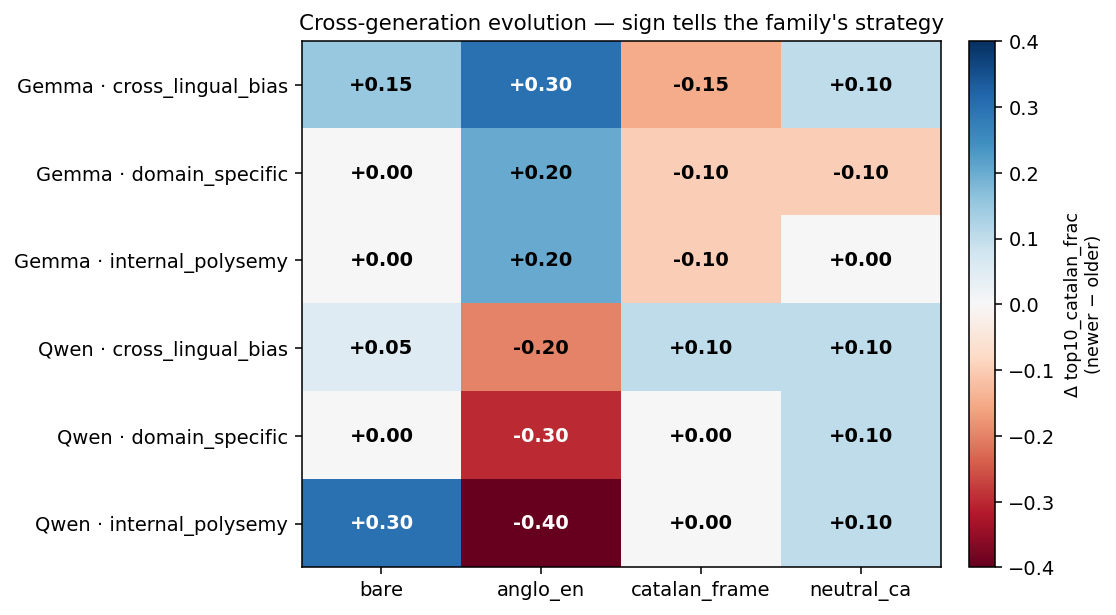
\includegraphics[width=\linewidth]{cross_generation_heatmap.png}
  \caption{$\text{top10\_catalan\_frac}(\text{newer}) -
  \text{top10\_catalan\_frac}(\text{older})$. Blue = the newer model places
  the concept more Catalan; red = it regressed. The two families move in
  opposite directions.}
  \label{fig:crossgen}
\end{figure}

\subsection{``Coca is not cocaine'' --- the title case}\label{sec:results-coca}

\paragraph{Under \code{anglo\_en}} ---\emph{``Once upon a time, there was a
coca who lived in the enchanted forest''}--- \textbf{Salamandra 7B places 9 of
10} nearest anchors in the noise cluster, ALIA-40B places 8, and Mistral Small
24B / Qwen 3.5 4B / Salamandra 2B place 7 each. Two outliers: Gemma 4 E2B and
DeepSeek 67B-base place \textbf{zero} noise anchors --- DeepSeek's top-3 is
\emph{enchanted forest, fairy, princess}, drifting cleanly into the fairy-tale
cluster instead (pure \Ftwo{}).

\paragraph{Under \code{bare}} (no carrier sentence) the effect persists: 7
noise hits on ALIA-40B, Mistral Small 24B and Salamandra 2B; 6 on DeepSeek
67B, Gemma 2, Qwen 2 and Salamandra 7B; and 0 only on Gemma 4 E2B. This is what
\emph{structural} means in the decision rule: the collision is a property of
where \concept{coca} lives in latent space, not induced by an English
scaffold.

\paragraph{Under \code{catalan\_frame}} noise drops to 0 on three models
(DeepSeek 67B, Gemma 4 E2B, Qwen 3.5 4B) and to 1 on Gemma 4 26B and Mistral
Small 24B (only \emph{Coca-Cola} survives); Gemma 4 26B's top-3 becomes
\emph{plaça, enxaneta, ajuntament}. The collision is rescuable, but only by a
strong native frame, and the rescue depth is family-dependent: the Salamandra
family and ALIA still carry 3--6 noise neighbours under \code{catalan\_frame},
the cleanest evidence that intentional Catalan training does not, by itself,
dissolve the \Fone{} collision.

\begin{figure}[t]
  \centering
  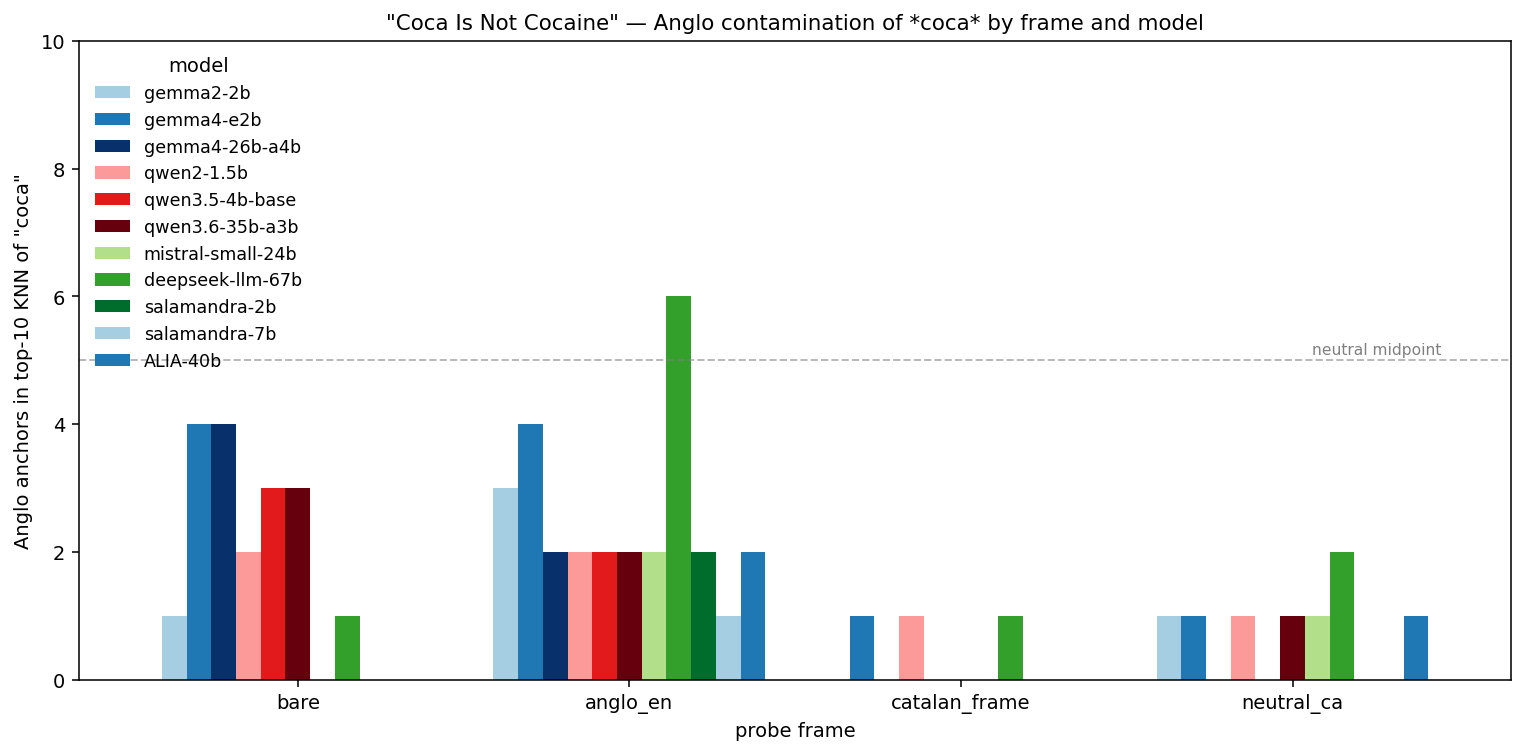
\includegraphics[width=\linewidth]{focus_coca_bar.png}
  \caption{Anglo-anchor count (blue side of the binary \code{bias\_ratio}) in
  the top-10 KNN of \concept{coca} per $(\text{model},\text{frame})$.
  Complement to Figure~\ref{fig:coca}: together they tell which cluster
  catches \concept{coca} when it drifts and which frame rescues it.}
  \label{fig:coca-bar}
\end{figure}

\begin{figure*}[t]
  \centering
  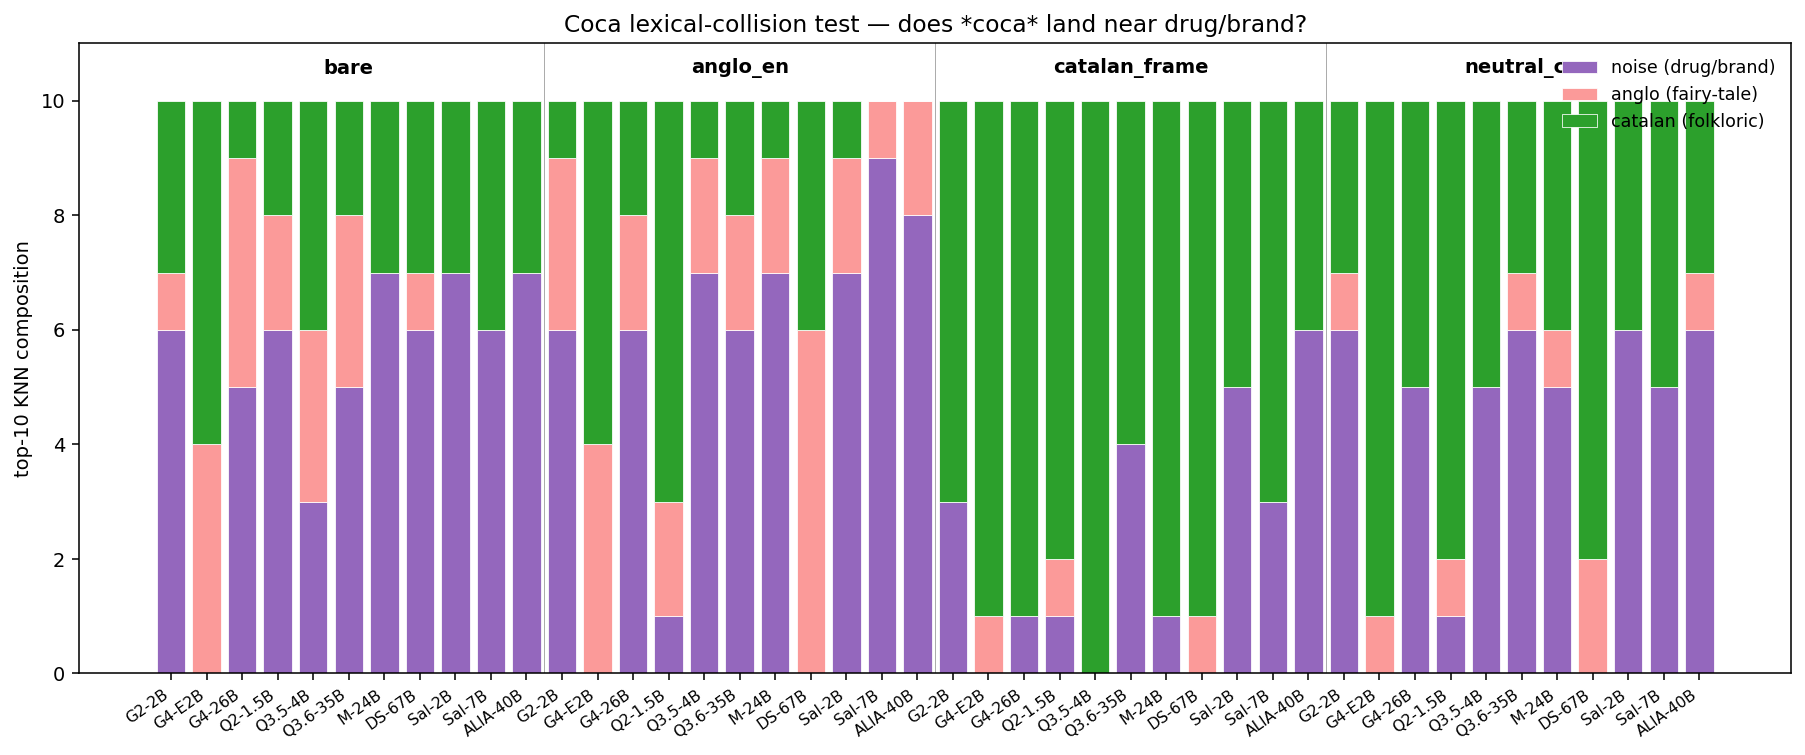
\includegraphics[width=0.86\textwidth]{coca_lexical_collision.png}
  \caption{Purple = noise-cluster (drug / brand / beverage) hits in the top-10
  KNN of \concept{coca} per $(\text{model},\text{frame})$. The pre-registered
  threshold $n_{\text{noise}} \geq 2$ outside \code{anglo\_en} returns the
  strongly supported (structural) branch on ten of eleven models.}
  \label{fig:coca}
\end{figure*}

\begin{table*}[t]
  \centering
  \small
  \renewcommand{\arraystretch}{1.18}
  \resizebox{\textwidth}{!}{%
  \begin{tabular}{@{}lllll@{}}
    \toprule
    \textbf{Model} & \code{bare} & \code{anglo\_en} & \code{catalan\_frame} & \code{neutral\_ca} \\
    \midrule
    ALIA-40b          & cocaine, Coca-Cola, caffeine & cocaine, Coca-Cola, soda          & Coca-Cola, cocaine, soda     & cocaine, Coca-Cola, soda \\
    deepseek-llm-67b  & Coca-Cola, coke, soda        & enchanted forest, fairy, princess & cercavila, castellers, poble & enxaneta, plaça, grallers \\
    gemma2-2b         & Coca-Cola, coke, soda        & Coca-Cola, coke, soda             & Coca-Cola, coke, cobla       & Coca-Cola, coke, cocaine \\
    gemma4-26b-a4b    & coke, caffeine, soda         & Coca-Cola, cocaine, coke          & plaça, enxaneta, ajuntament  & Coca-Cola, cocaine, plaça \\
    gemma4-e2b        & cercavila, dwarf, dungeon    & enchanted forest, peasant, pessebre & enxaneta, plaça, pessebre   & pessebre, enxaneta, plaça \\
    mistral-small-24b & coke, cocaine, Coca-Cola     & Coca-Cola, coke, caffeine         & plaça, Coca-Cola, pessebre   & Coca-Cola, caffeine, coke \\
    qwen2-1.5b        & coke, soda, caffeine         & cercavila, Coca-Cola, enxaneta    & cercavila, enxaneta, Coca-Cola & cercavila, enxaneta, Coca-Cola \\
    qwen3.5-4b-base   & cercavila, soda, pilar       & Coca-Cola, cocaine, coke          & plaça, cobla, colla          & plaça, Coca-Cola, diada \\
    qwen3.6-35b-a3b   & Coca-Cola, coke, soda        & Coca-Cola, cocaine, coke          & Coca-Cola, coke, cocaine     & Coca-Cola, cocaine, coke \\
    salamandra-2b     & cocaine, Coca-Cola, caffeine & cocaine, Coca-Cola, caffeine      & Coca-Cola, cocaine, cobla    & cocaine, Coca-Cola, caffeine \\
    salamandra-7b     & cocaine, Coca-Cola, caffeine & cocaine, Coca-Cola, soda          & Coca-Cola, cocaine, cobla    & cocaine, Coca-Cola, caffeine \\
    \bottomrule
  \end{tabular}%
  }
  \caption{The three nearest neighbours of \concept{coca} per $(\text{model},
  \text{frame})$. \code{catalan\_frame} is the only frame that consistently
  rescues the concept toward the festive neighbourhood (\emph{plaça,
  enxaneta, cercavila}).}
  \label{tab:coca-top3}
\end{table*}

\subsection{The Catalan-aware control (Salamandra/ALIA)}

The H6 verdict from the Catalan-aware extraction is that intentional Catalan
training does not, by itself, erase the \Fone{}/\Ftwo{}/\Fthree{} collisions.
The collision modes survive across the Salamandra family up to ALIA-40B,
suggesting they are properties of the \textbf{contextualized-embedding
pipeline} (tokenization, mean-pooling, training-objective geometry) rather
than of the data mixture. Three of four pre-specified H6 sub-hypotheses were
falsified. \emph{Without the Salamandra/ALIA panel we could not have
distinguished the data-mix hypothesis from the pipeline hypothesis}: it is the
indispensable causal control of this study.

\subsection{The five-method statistical-rigour suite}

Every model goes through five uniform additional analyses, all derivable from
the committed artifacts without retraining:
(1)~per-concept paired-bootstrap CI on $\Delta$ (Figure~\ref{fig:delta},
Table~\ref{tab:delta}); (2)~layer-depth $\times$ frame interaction
(Figure~\ref{fig:layerdepth}); (3)~Anglo-subcluster pull on the focus concepts
(Figure~\ref{fig:subcluster}); (4)~stratified-bootstrap CIs on the
model~$\times$~ambiguity\_type~$\times$~frame median table
(Figure~\ref{fig:strat}); and (5)~Procrustes cross-model alignment
(Figure~\ref{fig:procrustes}).

\begin{table}[t]
  \centering
  \small
  \setlength{\tabcolsep}{5pt}
  \begin{tabular}{@{}lrrr@{}}
    \toprule
    \textbf{Model} & \textbf{median $\Delta$} & \textbf{n robust} & \textbf{n total} \\
    \midrule
    gemma2-2b         & 0.020 & 56 & 56 \\
    gemma4-e2b        & 0.024 & 49 & 50 \\
    gemma4-26b-a4b    & 0.068 & 56 & 56 \\
    qwen2-1.5b        & 0.010 & 56 & 56 \\
    qwen3.5-4b-base   & 0.095 & 56 & 56 \\
    qwen3.6-35b-a3b   & 0.045 & 56 & 56 \\
    mistral-small-24b & 0.058 & 56 & 56 \\
    deepseek-llm-67b  & 0.034 & 56 & 56 \\
    salamandra-2b     & 0.039 & 56 & 56 \\
    salamandra-7b     & 0.035 & 56 & 56 \\
    ALIA-40b          & 0.046 & 56 & 56 \\
    \bottomrule
  \end{tabular}
  \caption{Median $\Delta$ per model and number of concepts whose 95\,\% CI
  excludes zero (n robust). All CIs are paired bootstrap. Qwen 3.5 4B has the
  highest median $\Delta$ (0.095): the most Catalan-frame-responsive. Qwen2
  1.5B the lowest (0.010).}
  \label{tab:delta}
\end{table}

\begin{figure}[t]
  \centering
  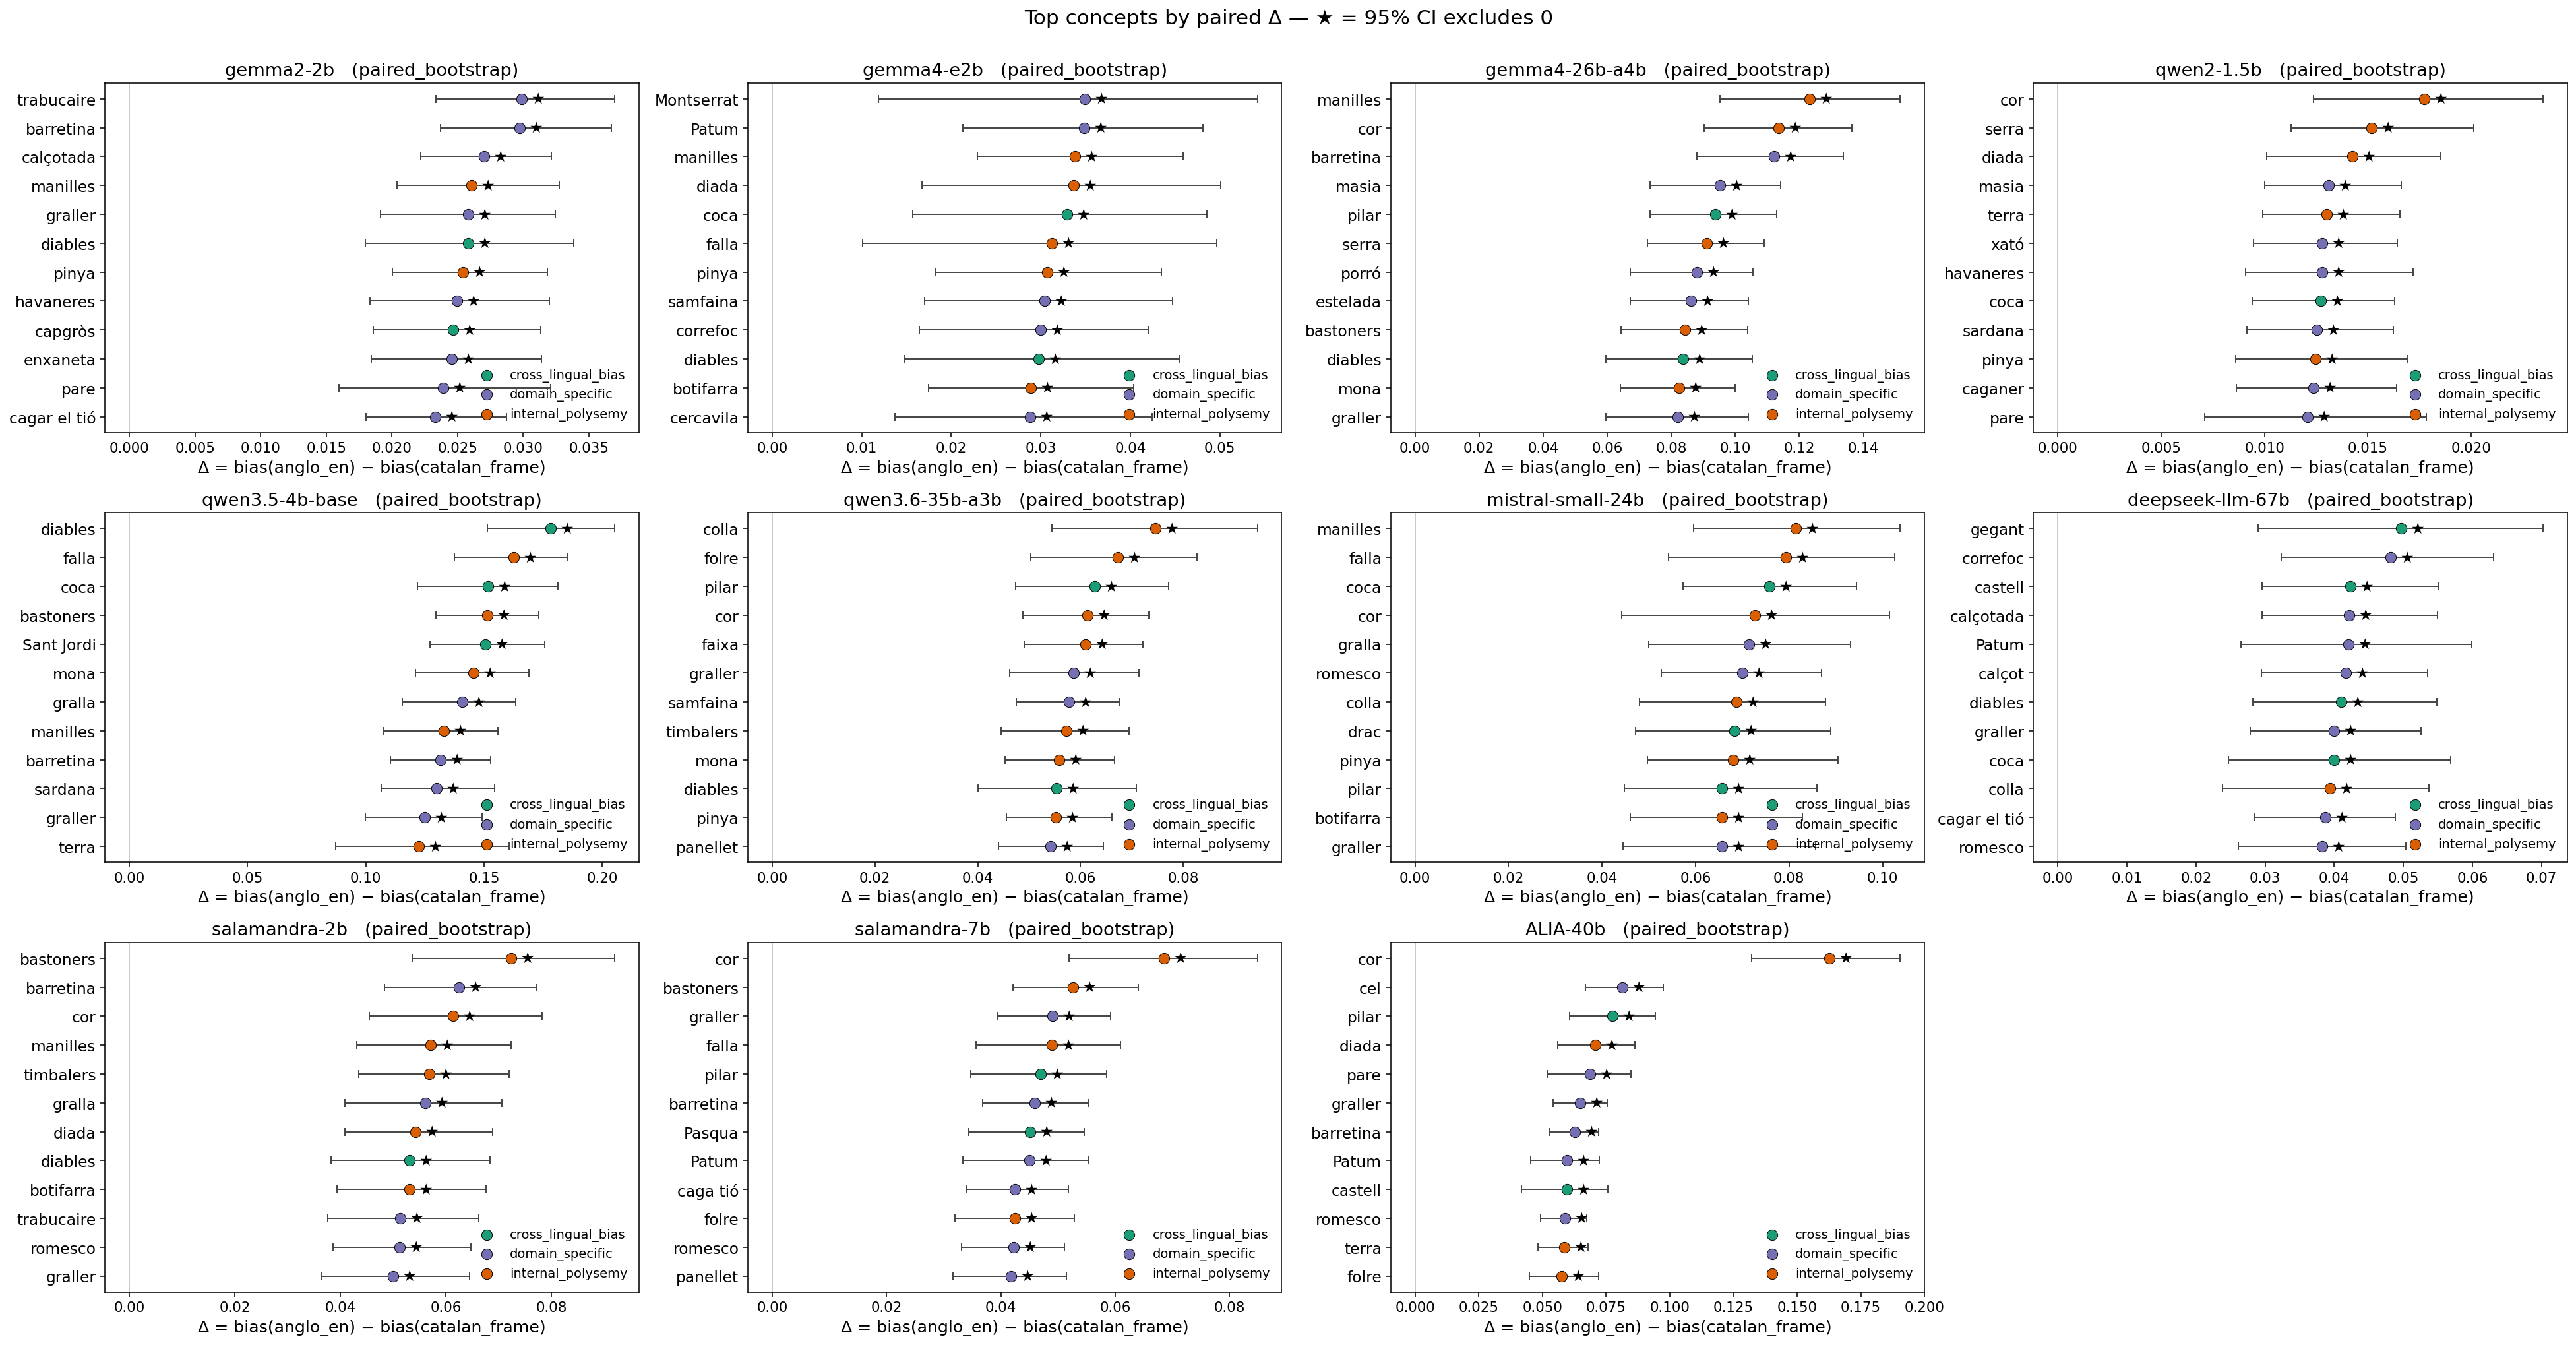
\includegraphics[width=\linewidth]{delta_forest.png}
  \caption{Forest plot of $\Delta(c) = \text{bias}(c,\text{anglo\_en}) -
  \text{bias}(c,\text{catalan\_frame})$ per concept with 95\,\% paired
  bootstrap CIs. Marked concepts have a CI excluding zero: robust evidence the
  Catalan frame changes the concept's geometry.}
  \label{fig:delta}
\end{figure}

\begin{figure*}[t]
  \centering
  \begin{subfigure}{0.48\textwidth}
    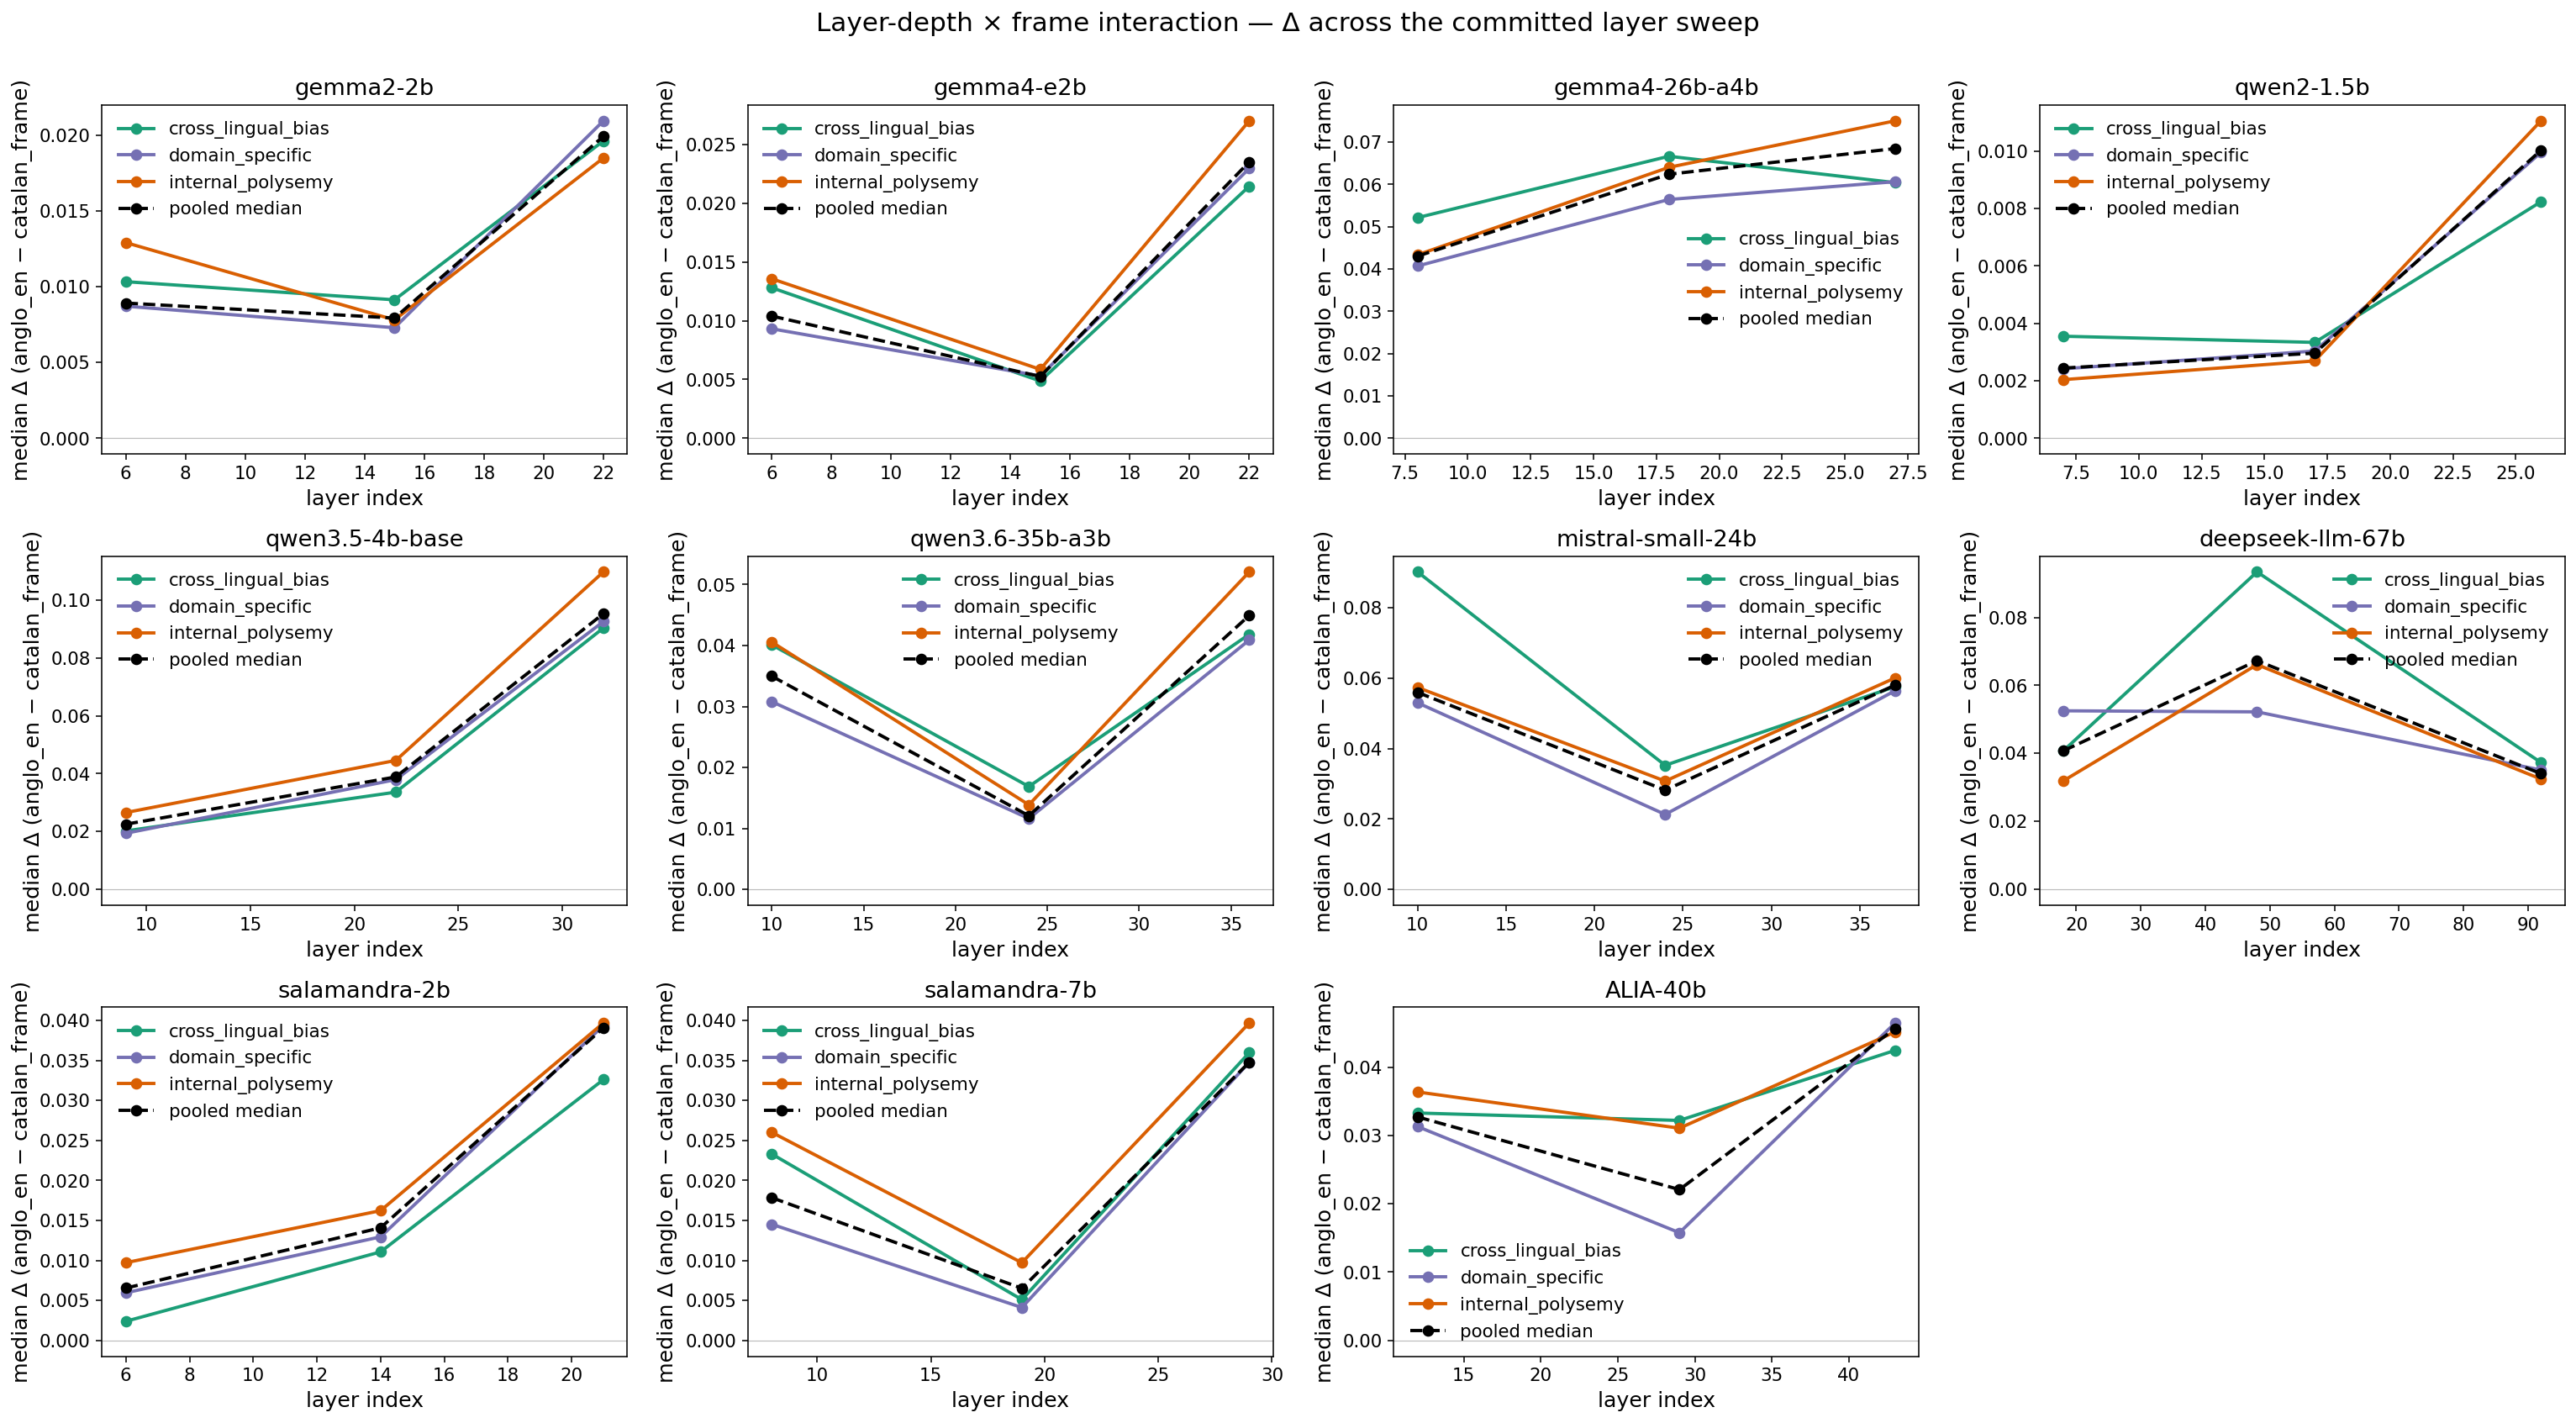
\includegraphics[width=\textwidth]{layer_depth_delta.png}
    \caption{Layer-depth $\times$ frame interaction.}
    \label{fig:layerdepth}
  \end{subfigure}\hfill
  \begin{subfigure}{0.48\textwidth}
    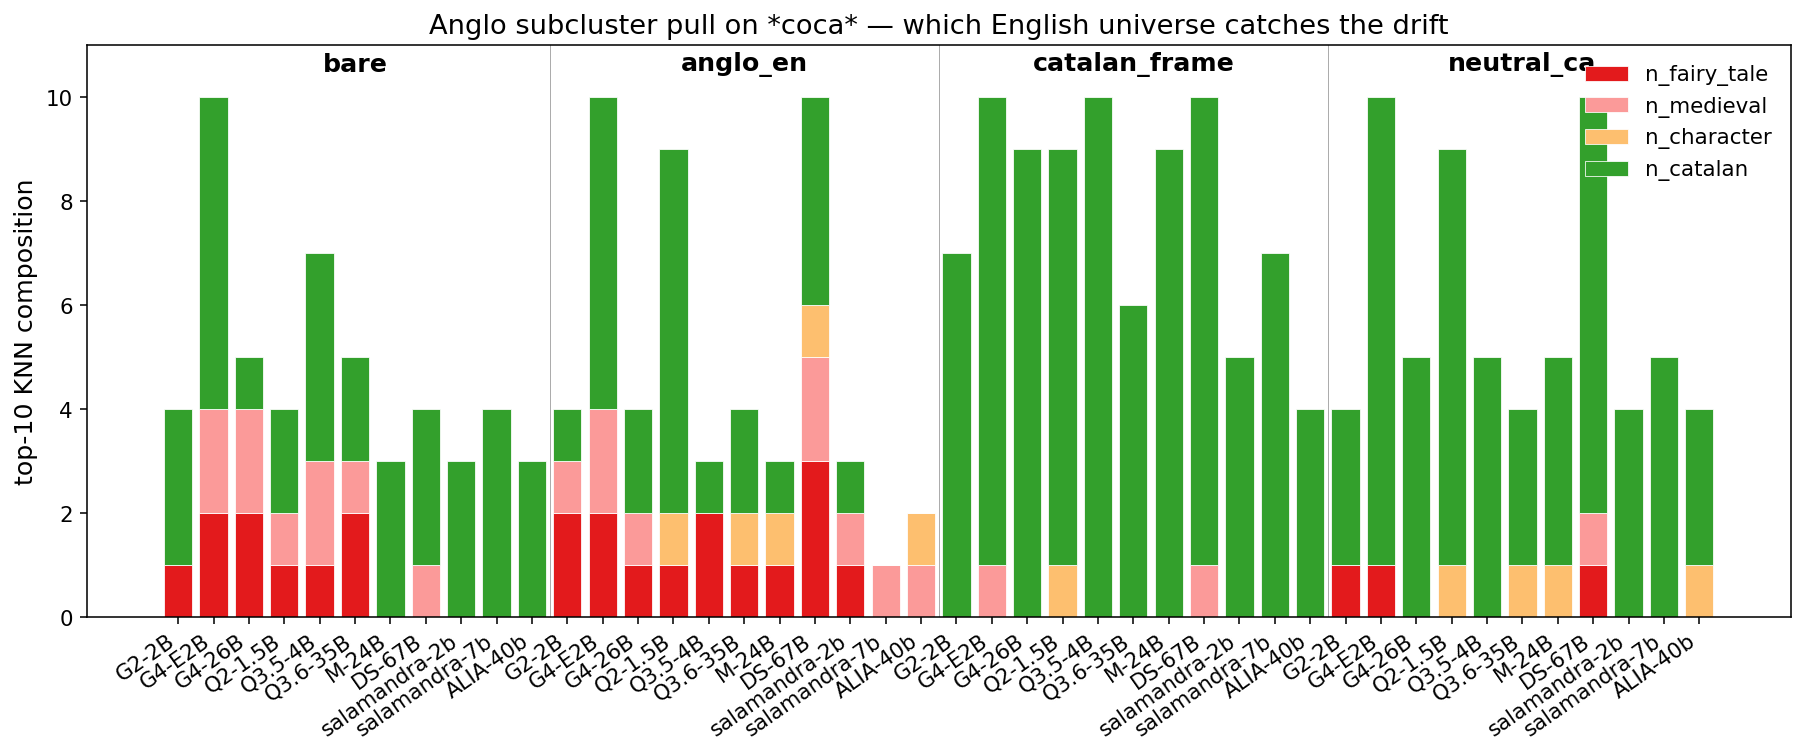
\includegraphics[width=\textwidth]{subcluster_coca.png}
    \caption{Anglo-subcluster pull on \concept{coca}.}
    \label{fig:subcluster}
  \end{subfigure}

  \medskip
  \begin{subfigure}{0.48\textwidth}
    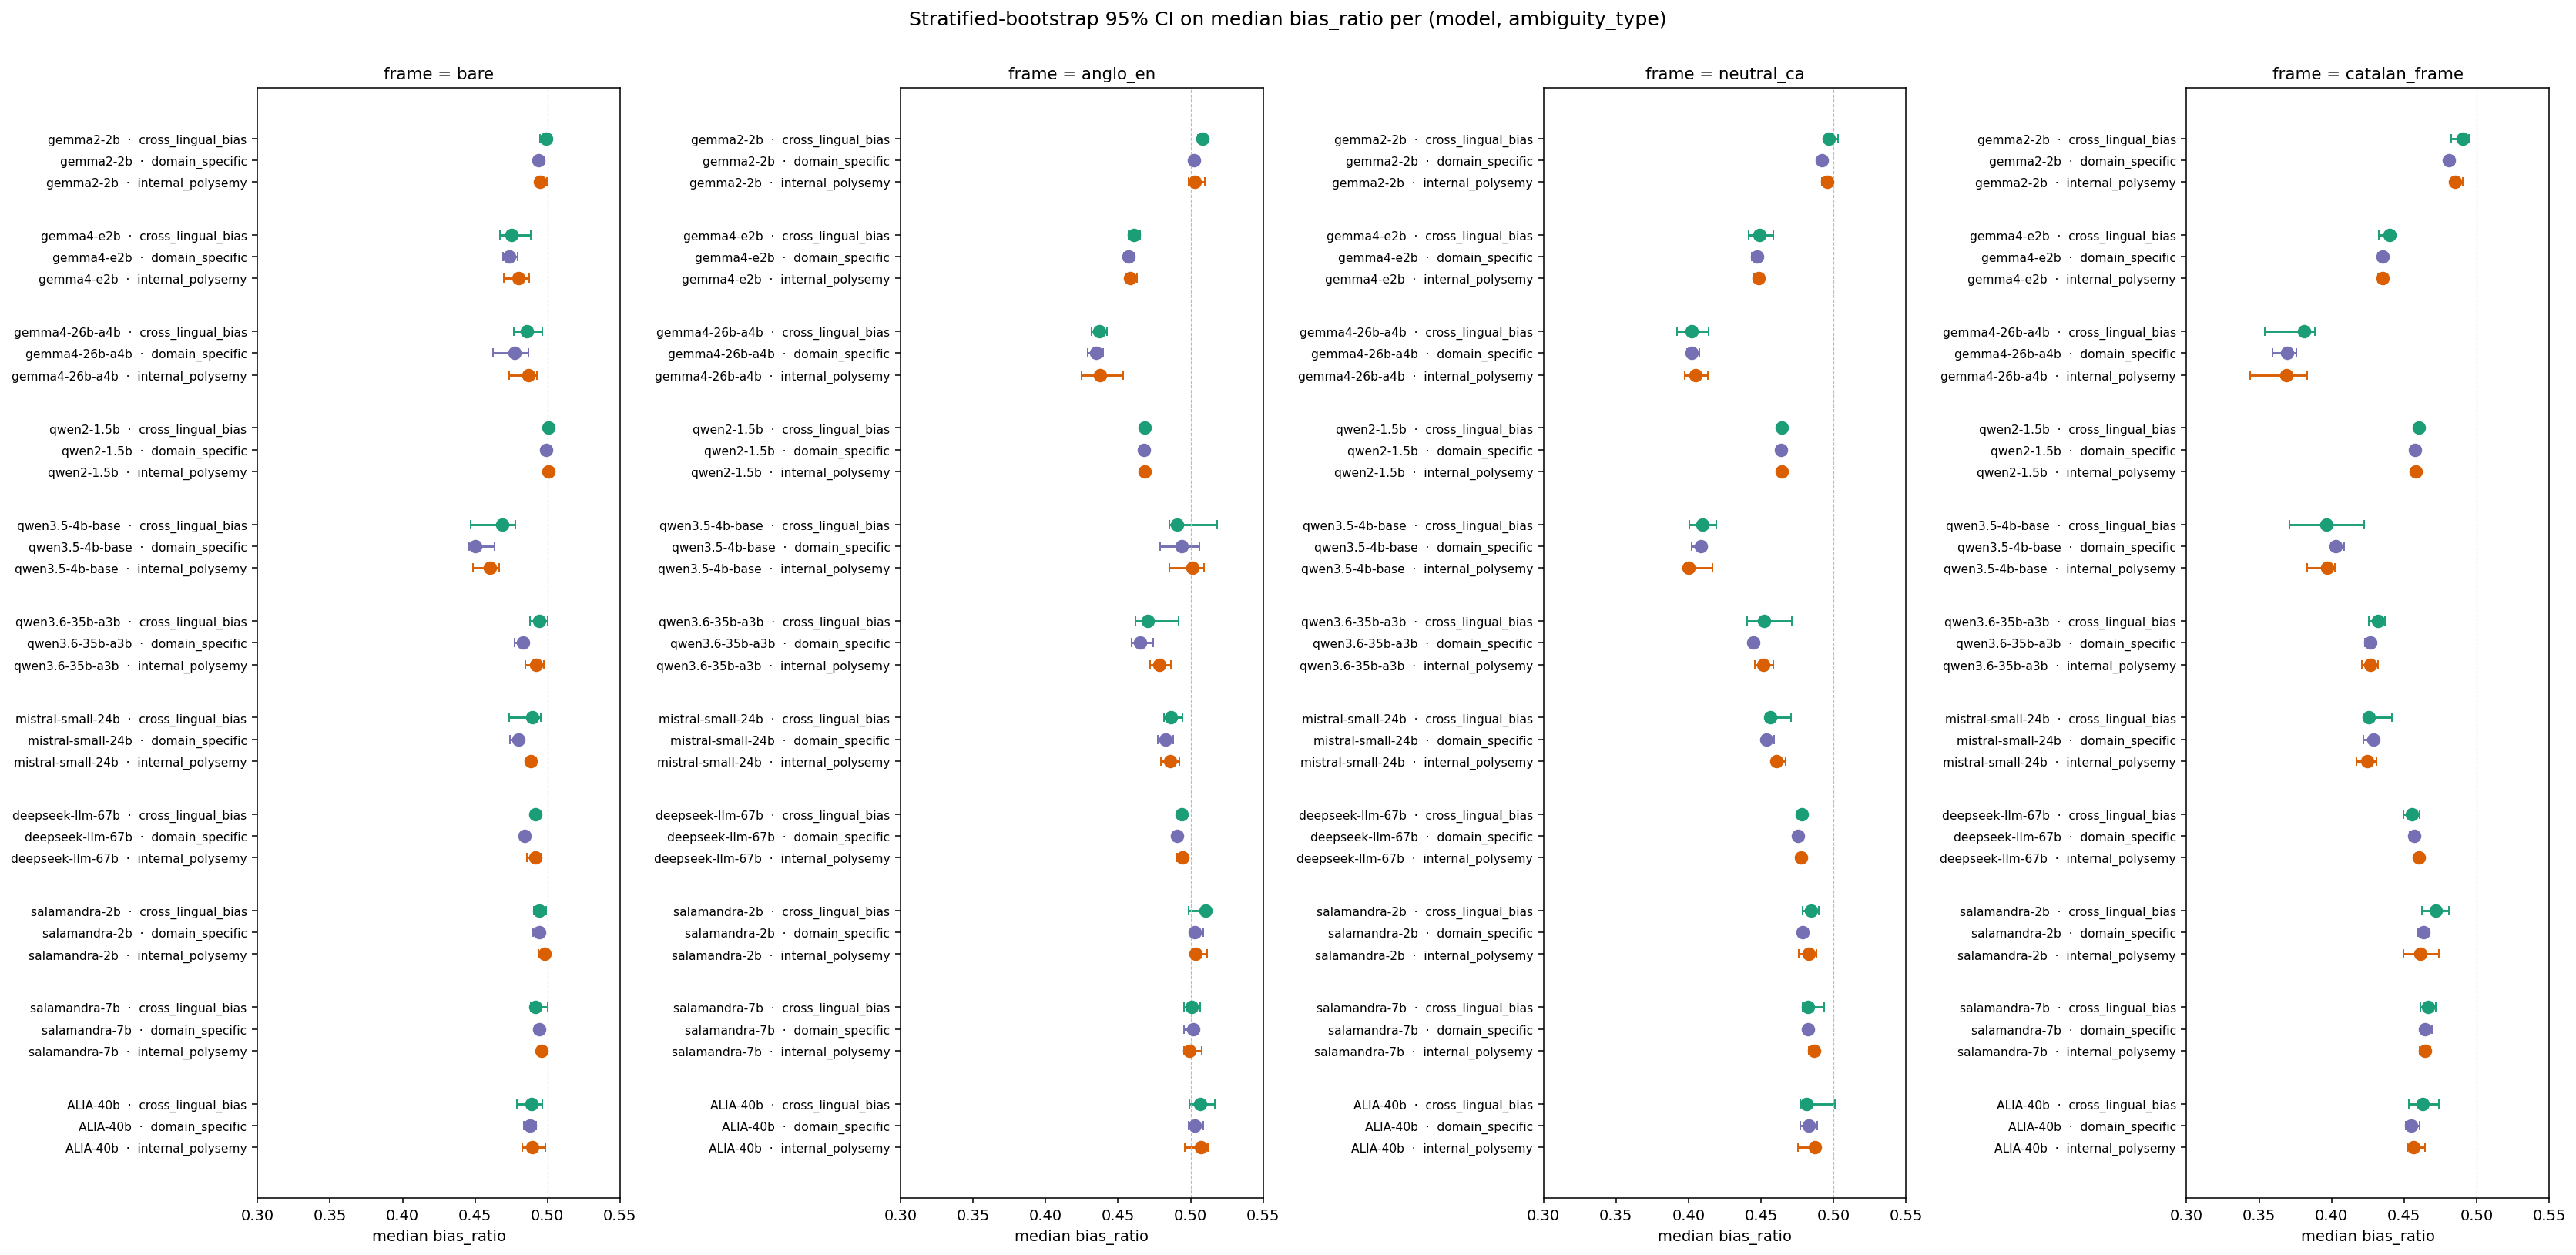
\includegraphics[width=\textwidth]{ambiguity_stratified_ci.png}
    \caption{Stratified-bootstrap CIs on the ambiguity-type medians.}
    \label{fig:strat}
  \end{subfigure}\hfill
  \begin{subfigure}{0.48\textwidth}
    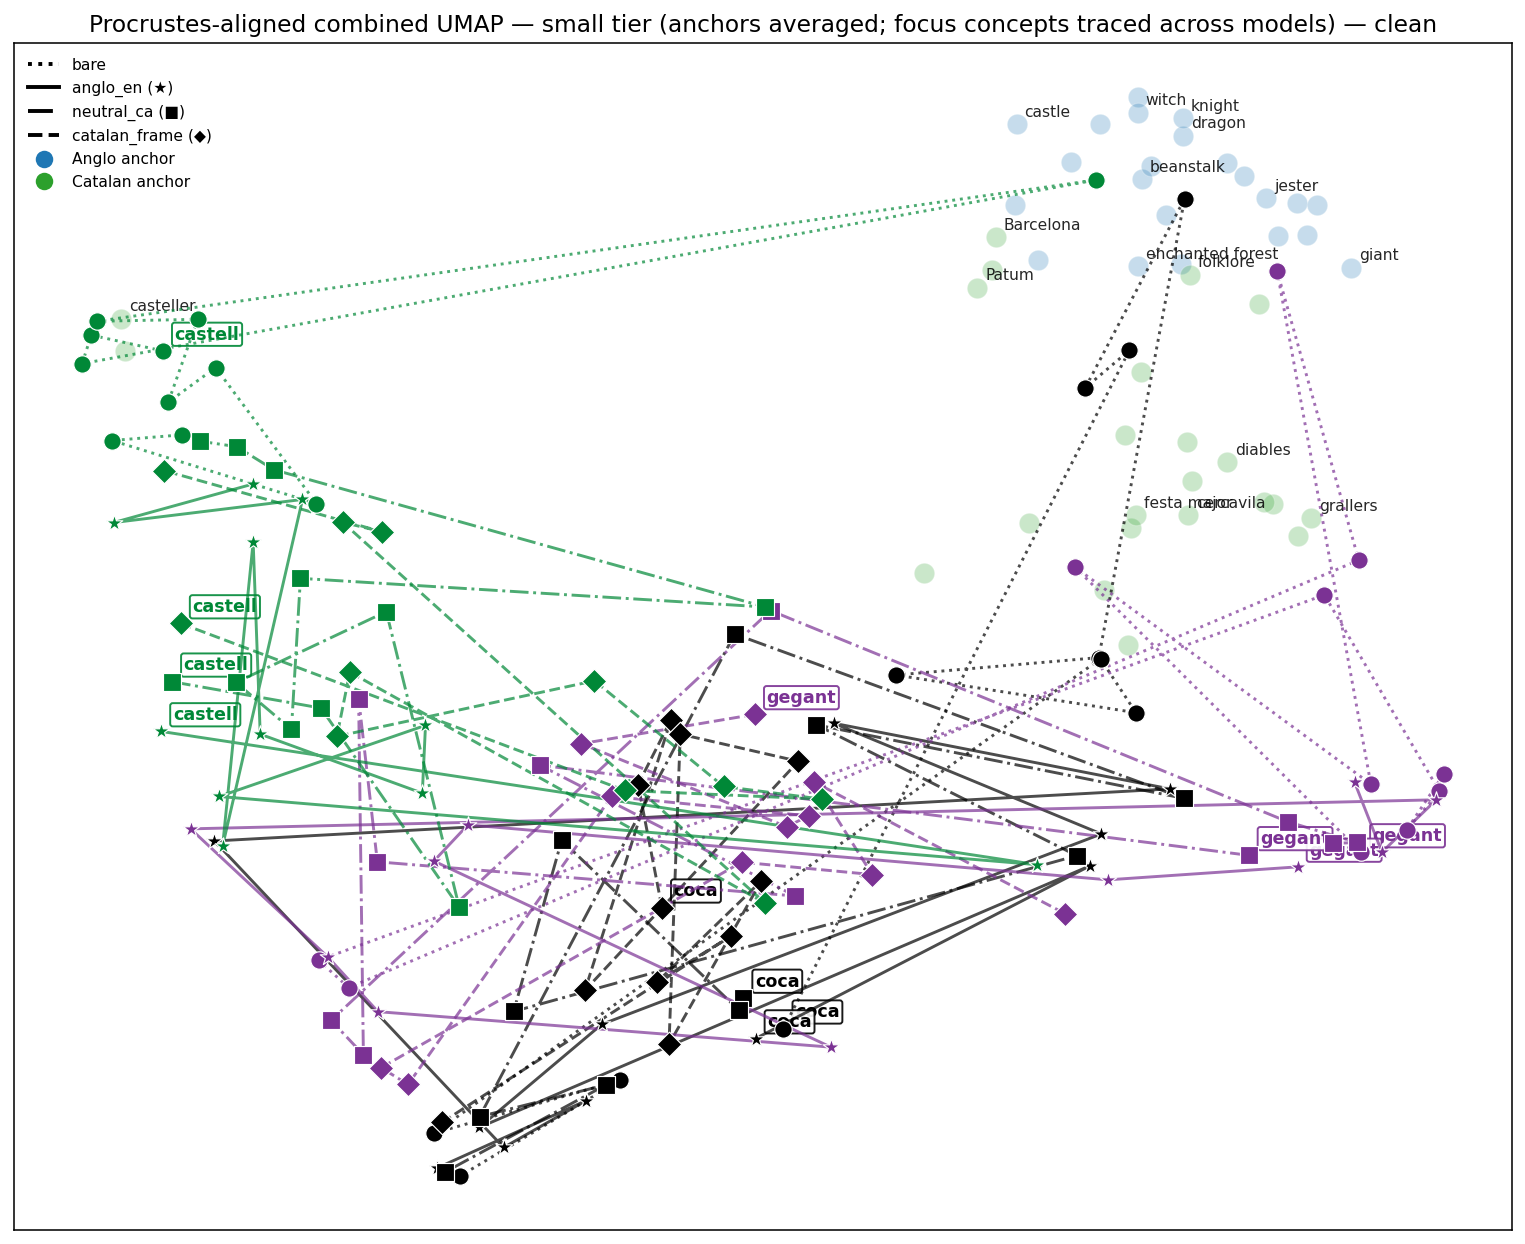
\includegraphics[width=\textwidth]{procrustes_combined_umap.png}
    \caption{Procrustes alignment across the small-tier models.}
    \label{fig:procrustes}
  \end{subfigure}
  \caption{The statistical-rigour suite. (a) whether the rescue happens early,
  mid or late in the stack; (b) which English universe (fairy-tale / medieval
  / character) catches \concept{coca} when it drifts; (c)
  \code{cross\_lingual\_bias} has only 10 concepts, so its medians carry the
  widest CIs by design; (d) focus concepts traced as polylines across the
  chronologically-aligned small-tier models.}
  \label{fig:suite}
\end{figure*}

% ---------------------------------------------------------------
\section{Discussion}\label{sec:discussion}
% ---------------------------------------------------------------

Read the \code{domain\_specific} (\Ftwo{}) stratum first: if
\concept{cercavila}, \concept{correfoc}, \concept{panellet} or
\concept{casteller} still sit closer to \emph{giant / jester / enchanted
forest} than to \emph{festa major / grallers / diables} --- even under a
native Catalan frame --- the pull is structural, not prompt-rescuable, and not
explained by any lexical cognate.

\code{cross\_lingual\_bias} (\Fone{}) items show the highest raw bias ratios,
but that number is confounded with the cognate meaning of the Catalan word
itself. They should not be read as the headline but as the \emph{upper bound}
of how strong the pull can get when the lexical shortcut is available.

\code{internal\_polysemy} (\Fthree{}) items are a different story: a high bias
ratio on \code{bare} or \code{neutral\_ca} most likely reflects the dominant
mundane Catalan sense (pinecone, log, geological fault), not an English arrow.
The frame differential is the interesting datum: if \code{catalan\_frame}
pulls the vector back into the festive neighbourhood, we were seeing polysemy;
if not, even explicit Catalan festive context cannot override the default
sense.

The \code{anglo\_en}~$\leftrightarrow$~\code{catalan\_frame} differential is
therefore the key diagnostic: a large drop under \code{catalan\_frame} means
prompt-rescuable (the festive sense was retrievable, just not the default); no
drop means the Catalan frame cannot override the English anchor --- structural
anglification.

% ---------------------------------------------------------------
\section{Limitations}\label{sec:limitations}
% ---------------------------------------------------------------

\begin{itemize}[leftmargin=1.3em,itemsep=3pt,topsep=2pt]
  \item \textbf{Mean-pooling over subwords} smears multi-token concepts
        (\concept{pa amb tomàquet}, \concept{caga tió}). A per-subword vector
        probe is queued for a future revision.
  \item \textbf{Hand-curated anchor lists} (22 / 23 / 13 entries): results are
        sensitive to that curation.
  \item \textbf{Cross-model raw cosines are not directly comparable.} The only
        surviving within-study comparisons are the normalized
        \code{bias\_ratio}, the rank-based \code{top10\_catalan\_frac}, and the
        Procrustes alignment (small tier only).
  \item \textbf{Layer-selection circularity}, mitigated by reporting every
        metric across the three layers and by the per-concept paired-bootstrap
        CI.
  \item \textbf{Quantization is excluded a priori} (bf16 only): this is what
        excludes DeepSeek-V3 (671B) and V4-Flash (584B); the dense
        DeepSeek-LLM-67B-Base does fit on a single H200.
  \item \textbf{Base variants only} (no instruct); instruct comparisons would
        require a separate study.
  \item \textbf{One language.} The methodology is language-independent; a
        15-concept replication in Occitan or Aragonese is queued.
\end{itemize}

\paragraph{What this study does not claim.} That a Catalan-aware model is
\emph{worse} than a general-purpose one (the H6 verdict is that Catalan
training does not cancel the inference-time requirement of a Catalan carrier
prompt, not that Salamandra/ALIA is worse than Gemma); that the title-test
result generalizes beyond \concept{coca}; nor that the operational
recommendation (``supply a Catalan carrier prompt'') solves the deployment
problem --- it rescues retrieval-style probes but says nothing about
generation quality, factual accuracy, or downstream tasks.

% ---------------------------------------------------------------
\section{Conclusions}\label{sec:conclusions}
% ---------------------------------------------------------------

\begin{enumerate}[leftmargin=1.4em,itemsep=4pt,topsep=2pt]
  \item \textbf{The \Fone{}/\Ftwo{}/\Fthree{} taxonomy is necessary.} Under
        \code{anglo\_en} on Qwen 3.5 4B the pooled median
        \code{top10\_catalan\_frac} is 0.50 --- a reader scanning a single
        number would conclude the model is unbiased. Stratifying reveals three
        stories inside that pool: \Fone{} = 0.55, \Ftwo{} = 0.50, \Fthree{} =
        0.40. The right intervention for \Fthree{} is to teach the model that
        \concept{pinya} has a second sense that is not a pinecone, not that
        \concept{gegant} $\neq$ \emph{giant}.

  \item \textbf{The two families moved in opposite directions, and it survives
        at the large tier.} Gemma becomes context-invariant; Qwen becomes
        context-amplified. There is no global ``best LLM for Catalan'' --- it
        depends on whether the deployment can guarantee Catalan framing.

  \item \textbf{Scale is not the answer.} The biggest Qwen (3.6 35B-A3B) is
        less responsive to Catalan framing than the smaller Qwen 3.5 4B.
        ALIA-40B (Catalan-aware) has the deepest drop and the strongest native
        response: what matters is the multilingual pretraining diet
        \emph{combined with} inference-time framing, not size.

  \item \textbf{``Coca is not cocaine'' is grounded by the metric, not the
        metaphor.} The pre-registered test ($n_{\text{noise}} \geq 2$ in the
        top-10 KNN of \concept{coca}, outside \code{anglo\_en}) returns the
        strongly supported (structural) branch on ten of eleven models. The
        sole exception is Gemma 4 E2B, which drifts into the Anglo fairy-tale
        cluster instead (\Ftwo{} catches it, the title test misses it). The
        \Fone{} reading is a literal property of latent space; the rescue is
        possible but only with a strong native frame, and its depth is
        family-dependent --- the Catalan-aware control tier carries the
        heaviest residual noise.
\end{enumerate}

\paragraph{Practical recommendation.} The consequence is complementary to any
pretraining strategy: \textbf{supply Catalan context in the inference-time
prompt}, which works equally well for every model in the panel,
general-purpose or Catalan-aware.

% ---------------------------------------------------------------
\section*{Data and code availability}
% ---------------------------------------------------------------
\addcontentsline{toc}{section}{Data and code availability}

The code (MIT), the hand-curated CSVs (CC-BY 4.0), all figures and extraction
artifacts are public at
\url{https://github.com/xaviviro/coca-is-not-cocaine}. The full methodological
memo (in Catalan) is \code{metodologia.pdf} in the repository.

\balance
% ---------------------------------------------------------------
\begin{thebibliography}{99}
\small
% ---------------------------------------------------------------

\bibitem[Bolukbasi et al.(2016)]{bolukbasi2016}
T.~Bolukbasi, K.-W.~Chang, J.~Zou, V.~Saligrama, A.~Kalai.
\newblock Man is to computer programmer as woman is to homemaker? Debiasing
  word embeddings.
\newblock NeurIPS 2016. \href{https://arxiv.org/abs/1607.06520}{arXiv:1607.06520}.

\bibitem[Dettmers et al.(2022)]{dettmers2022}
T.~Dettmers, M.~Lewis, Y.~Belkada, L.~Zettlemoyer.
\newblock LLM.int8(): 8-bit matrix multiplication for transformers at scale.
\newblock NeurIPS 2022. \href{https://arxiv.org/abs/2208.07339}{arXiv:2208.07339}.

\bibitem[Li et al.(2023)]{li2023}
S.~Li, B.~Shafiq, P.~Mathur, S.~Roy.
\newblock GeoMLAMA: Geographical and cultural biases in multilingual
  pre-trained language models.
\newblock \href{https://arxiv.org/abs/2205.12247}{arXiv:2205.12247}.

\bibitem[Naous et al.(2024)]{naous2024}
T.~Naous, M.~J.~Ryan, A.~Ritter, W.~Xu.
\newblock Having beer after prayer? Measuring cultural bias in large language
  models.
\newblock ACL 2024. \href{https://arxiv.org/abs/2305.14456}{arXiv:2305.14456}.

\bibitem[Rystrøm et al.(2025)]{rystrom2025}
J.~Rystrøm, H.~R.~Kirk, S.~Hale.
\newblock Multilingual $\neq$ multicultural.
\newblock \href{https://arxiv.org/abs/2502.16534}{arXiv:2502.16534}.

\bibitem[Tao et al.(2024)]{tao2024}
Y.~Tao, O.~Viberg, R.~S.~Baker, R.~F.~Kizilcec.
\newblock Cultural bias and cultural alignment of large language models.
\newblock PNAS Nexus 2024. \href{https://arxiv.org/abs/2311.14096}{arXiv:2311.14096}.

\bibitem[Wang et al.(2023)]{wang2023}
W.~Wang, M.~Saar-Tsechansky, M.~Sun, S.~Wang.
\newblock Not all countries celebrate Thanksgiving: On the cultural dominance
  in large language models.
\newblock \href{https://arxiv.org/abs/2310.12481}{arXiv:2310.12481}.

\bibitem[Ada Lovelace Institute(2025)]{adalovelace2025}
Ada Lovelace Institute.
\newblock Tokenising culture: causes and consequences of cultural
  misalignment in LLMs. 2025.
\newblock \url{https://www.adalovelaceinstitute.org/blog/cultural-misalignment-llms/}.

\end{thebibliography}

\end{document}
